\chapter[]{\titleof{c3}}
\label{chap:3}
%
\begin{quote}
Hierarchies are powerful structures to model different levels of associations in the data. They can evolve over time in term of the relations between entities in the hierarchy and learning representations that are agnostic to these changes are not trivial. We can, however, take the horizontal and vertical dependencies in a hierarchy into account and learn highly separable representations for entities that are less variant to structural changes and more transferable over time. 
\end{quote}
%
\section{Introduction}
Hierarchy is an effective and common way of representing information, and many domains are naturally organized in a hierarchy. Organizing data in a hierarchical structure is valuable since it determines relationships in the data at different levels of resolution and picks out different categories relevant to each of the various layers of memberships.  
Besides that, using hierarchies is an effective way of representing the information as it eases the task of \emph{comparison}, which is a critical factor in analogical reasoning. For example, the problem of deciding whether two entities are analogous can be formalized as the problem of checking the level of abstraction at which these entities are instances of the same node in a hierarchy.

Taking advantage of the structure in a hierarchy requires modeling and representing entities, taking their relationship in the hierarchy into consideration. 
There are two types of dependencies in the hierarchies: i) \emph{Horizontal dependency}, which refers to the relations of entities in the same layer.  A simple example would be the dependency between siblings which have some commonalities in terms of being descendants of the same entity. ii) \emph{Vertical dependency}, which addresses the relations between ancestors and descendants in the hierarchy. For example the relation between root and other entities. 

Due to the existence of two\:-\:dimensional dependencies between entities in the hierarchy, modeling them regardless of their relationships might result in overlapping models that are not capable of making different entities distinguishable.  Learning representations with minimal overlap is one of the requirements for collision resistance systems and when the representations are not well\:-\:separated, classification and retrieval systems are less likely to work well~\citep{Lewis:1992}. 
Thus, \emph{two\:-\:dimensional separability}, i.e.\ \emph{horizontal and vertical separability}, is one of the key requirements of hierarchical classification.

In this chapter, we focus on one of our research questions:
\resq{c3}

We introduce \hswlms, which extends the idea of \swlms to the hierarchical structure. We assume that entities, like people, organizations, concepts, and ideologies are organized in a hierarchy, and for each entity, there are textual data associated with the entity with respect to the subhierarchy under the entity, where the data is generated only at the leaves of the hierarchy. Each entity, which is a node in the hierarchy, is represented by a specific probabilistic language model.

Given the hierarchical structure and the data associated with entities in the hierarchy, \achswlm iteratively sparsifies the representation of the entities by discarding features that are well explained by their ancestors, i.e., general features, as well as features that reflect the characteristics of individual descendants, i.e., specific features. This leads to representations for entities that are both vertically and horizontally separable, in terms of their position in the hierarchy, as they capture only the significant features of entities.

\begin{figure}[!t]
\centering
\tikzset{
every tree node/.style={align=center,anchor=north}
edge from parent/.style={very thick},
%edge from parent/.style=
%{draw, edge from parent path={(\tikzparentnode.south)
%-- +(0,-8pt)
%-| (\tikzchildnode)}},
blank/.style={draw=none}}
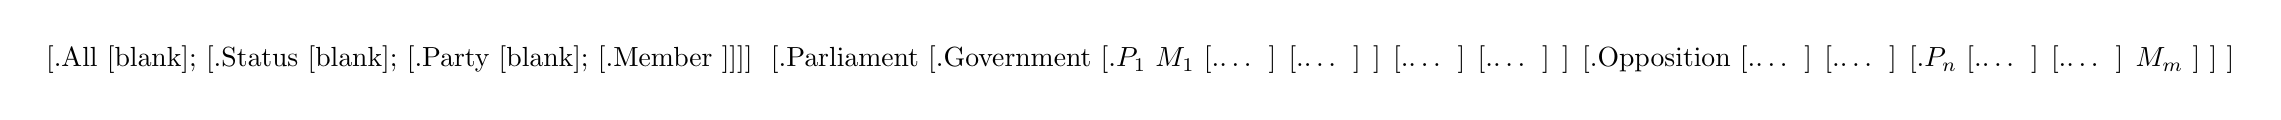
\begin{tikzpicture}[level distance = 30pt]
% \fontsize{7}{8}\selectfont
\matrix
{
\node{\Tree
    [.All  \edge[blank]; 
    [.Status  \edge[blank];
    [.Party \edge[blank]; 
    [.Member ]]]]};
&
\node{\Tree 
    [.Parliament
        [.Government
            [.$P_1$  $M_1$ [.{\dots} ] [.{\dots} ] ]
            [.{\dots} ]
            [.{\dots} ]
%            [.$P_n$  $M_1$ [.{\dots} ] $M_n$ ]
        ]
        [.Opposition 
%            [.$P_1$  $M_1$ [.{\dots} ]  $M_m$ ]
            [.{\dots} ]
            [.{\dots} ]
            [.$P_n$  [.{\dots} ] [.{\dots} ] $M_m$ ]
        ]
    ]};\\
};
\shrink
\end{tikzpicture}
\caption{\label{fig:ParHierarchy}Hierarchical relations in parliament.}
\end{figure}
As a concrete example, consider a simple hierarchy of a multi\:-\:party parliament as shown in Figure~\ref{fig:ParHierarchy}, which determines different categories relevant to the different layers of membership in the parliament.  We can associate an individual member of parliament by her speeches, a political party by their member's speeches, the opposition by the speeches of members of opposition parties, etc. 
In order to represent a party in this hierarchy, a proper model would show common characteristics of its members\:---\:not members of other parties (\emph{horizontal} separation), and capture the party's generic characteristics\:---\:not unique aspects of the current members captured in the individual member's layer or aspects of whether the party is in government or opposition captured in the status layer (\emph{vertical} separation).

\subsection{The Importance of Representational Separability}
The concept of \emph{separability} is of crucial importance especially when the task is not just ranking a set of items, but making a boolean decision about the labels of each item in the set.
Regarding this concern, \citet{Lewis:1995} has presented the Probability Threshold Principle (PTP), as a stronger version of the Probability Ranking Principle~\citep{Robertson:1977}, for binary classification, which discusses optimizing a threshold for separating items regarding their probability of class membership. 
PTP is a principle based on the separability in the score space. However, here we discuss separability in the data representation and later in this chapter we define a \emph{\ssp} as the counterpart of PTP in the feature space.
\begin{figure}[t]
% \makebox[\linewidth][c]{
\centering
\begin{subfigure}{0.49\textwidth}
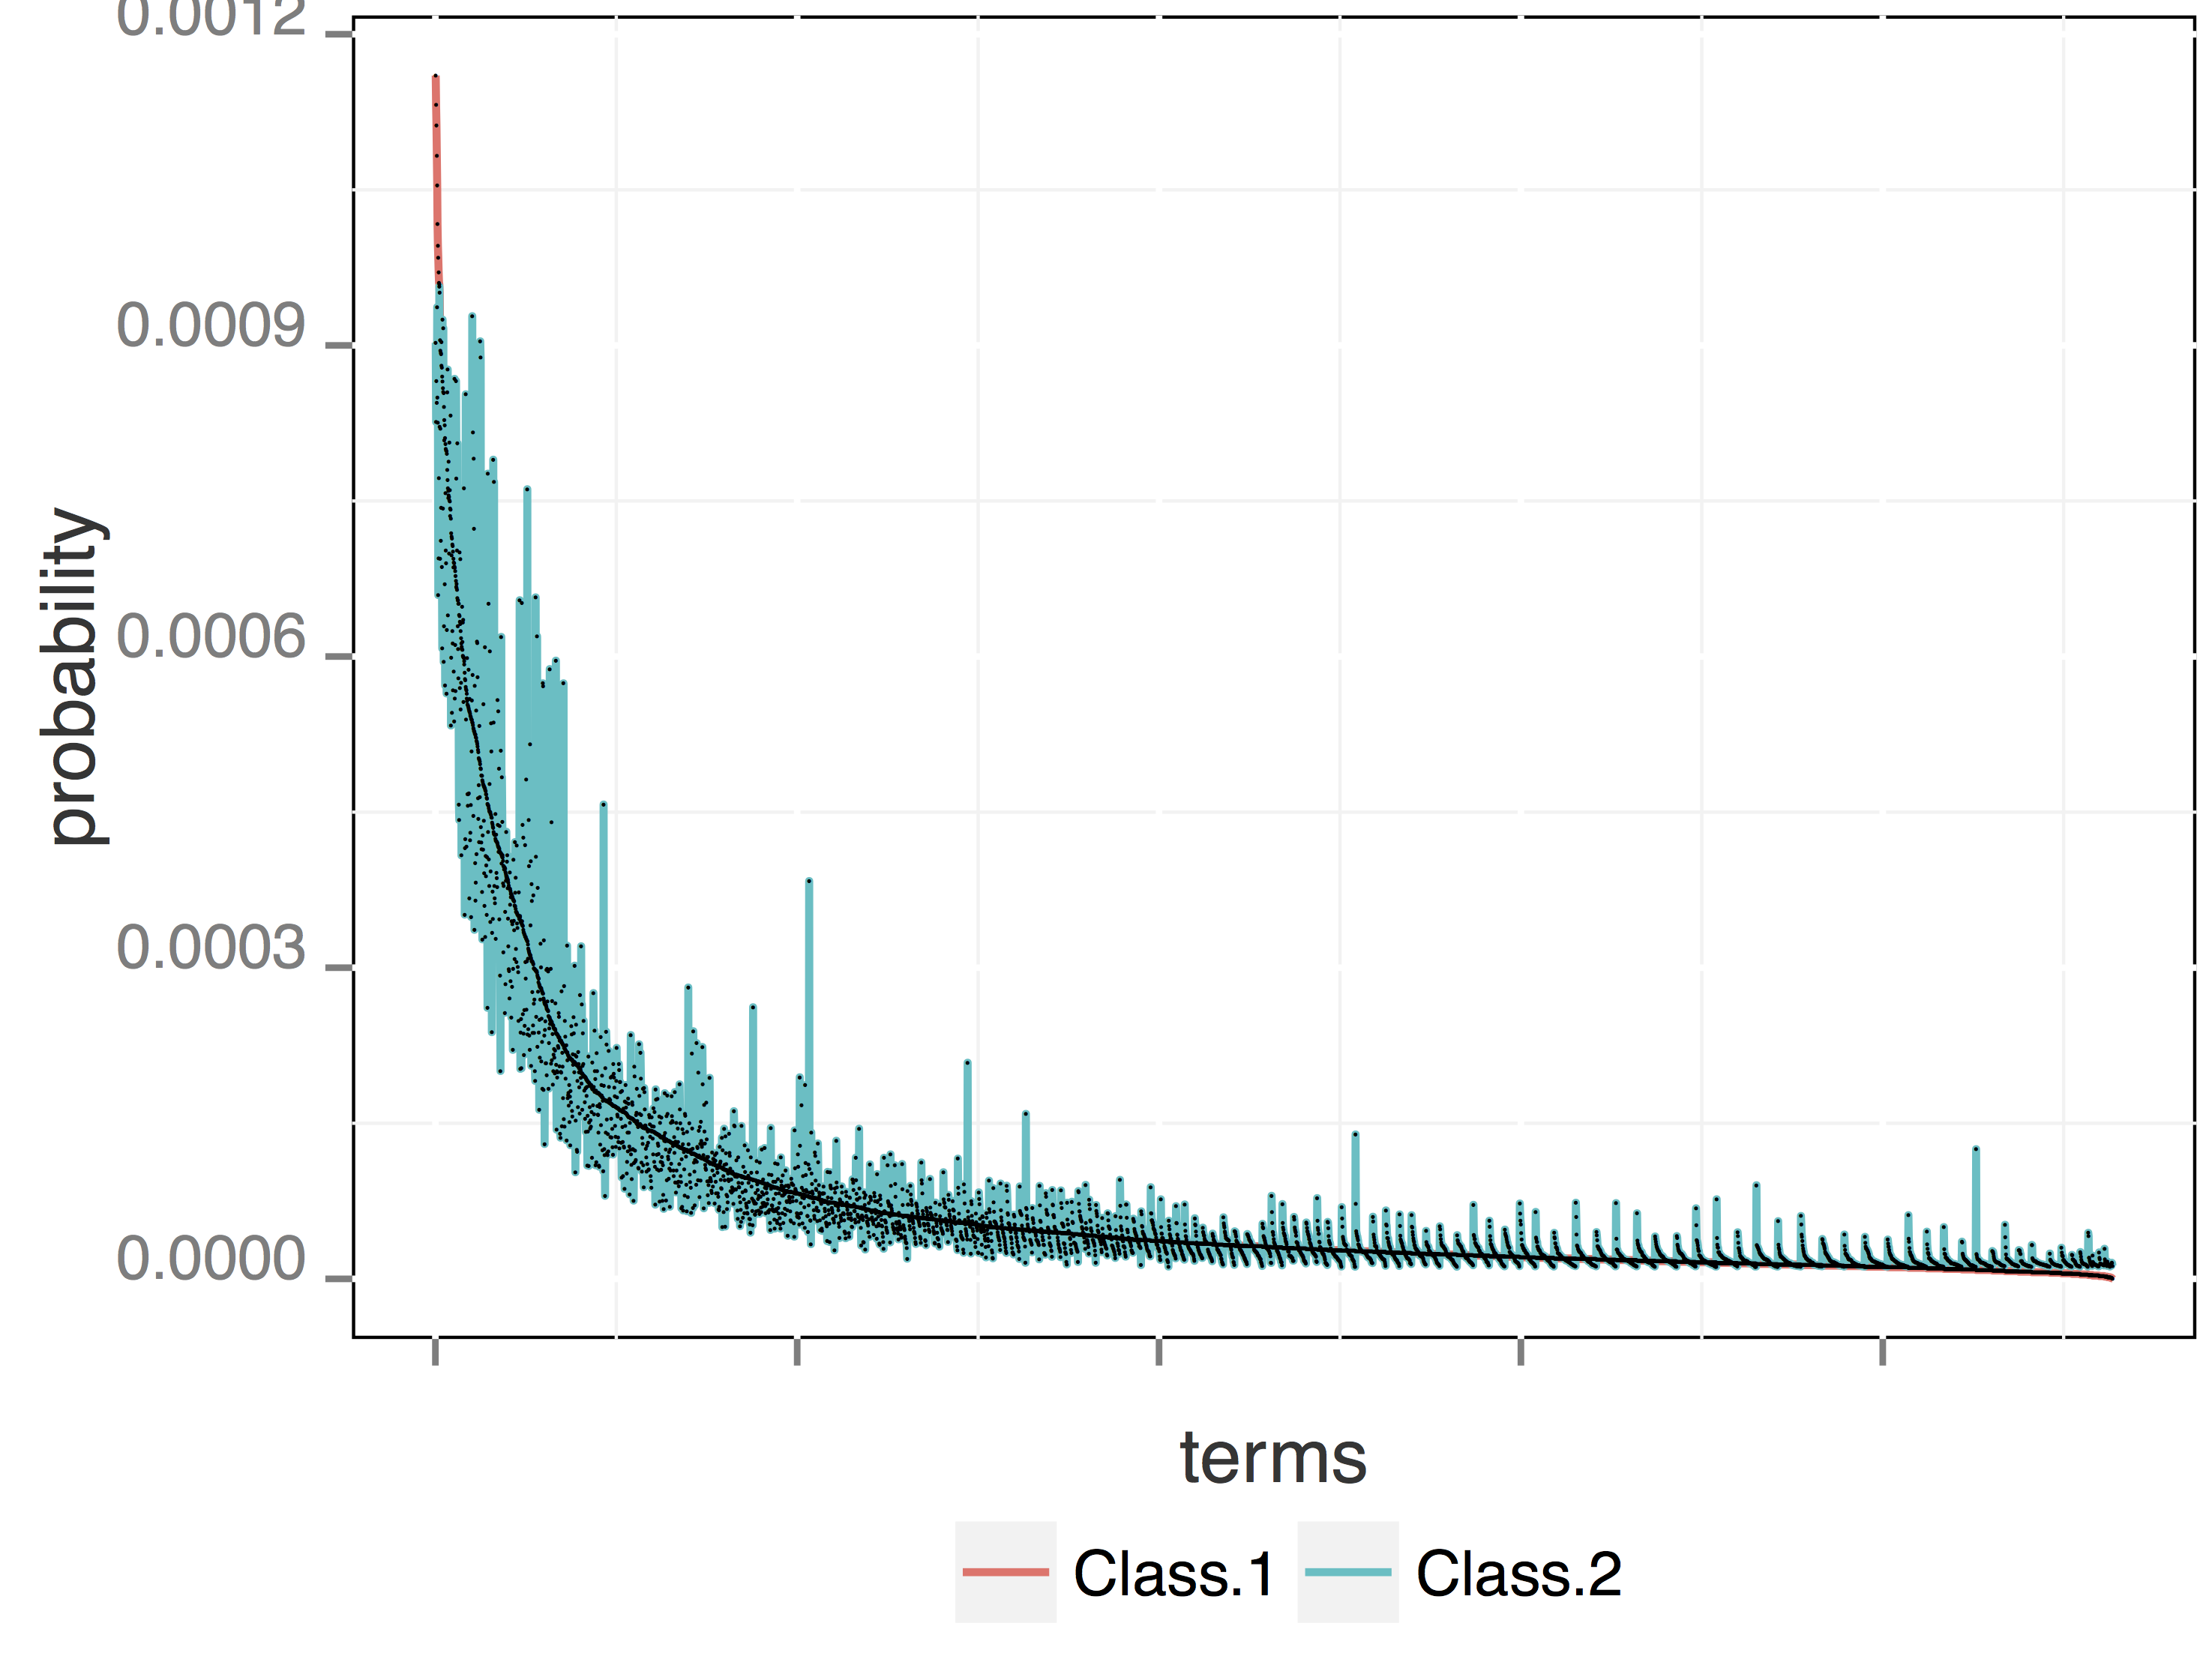
\includegraphics[width=\linewidth]{02-part-01/chapter-03/figs_and_tables/img_example-slm.png}
\caption{\label{fig:sep-slm} \scriptsize{A non-separable representation of data.}}
\end{subfigure}
\hfill
\begin{subfigure}{0.49\textwidth}
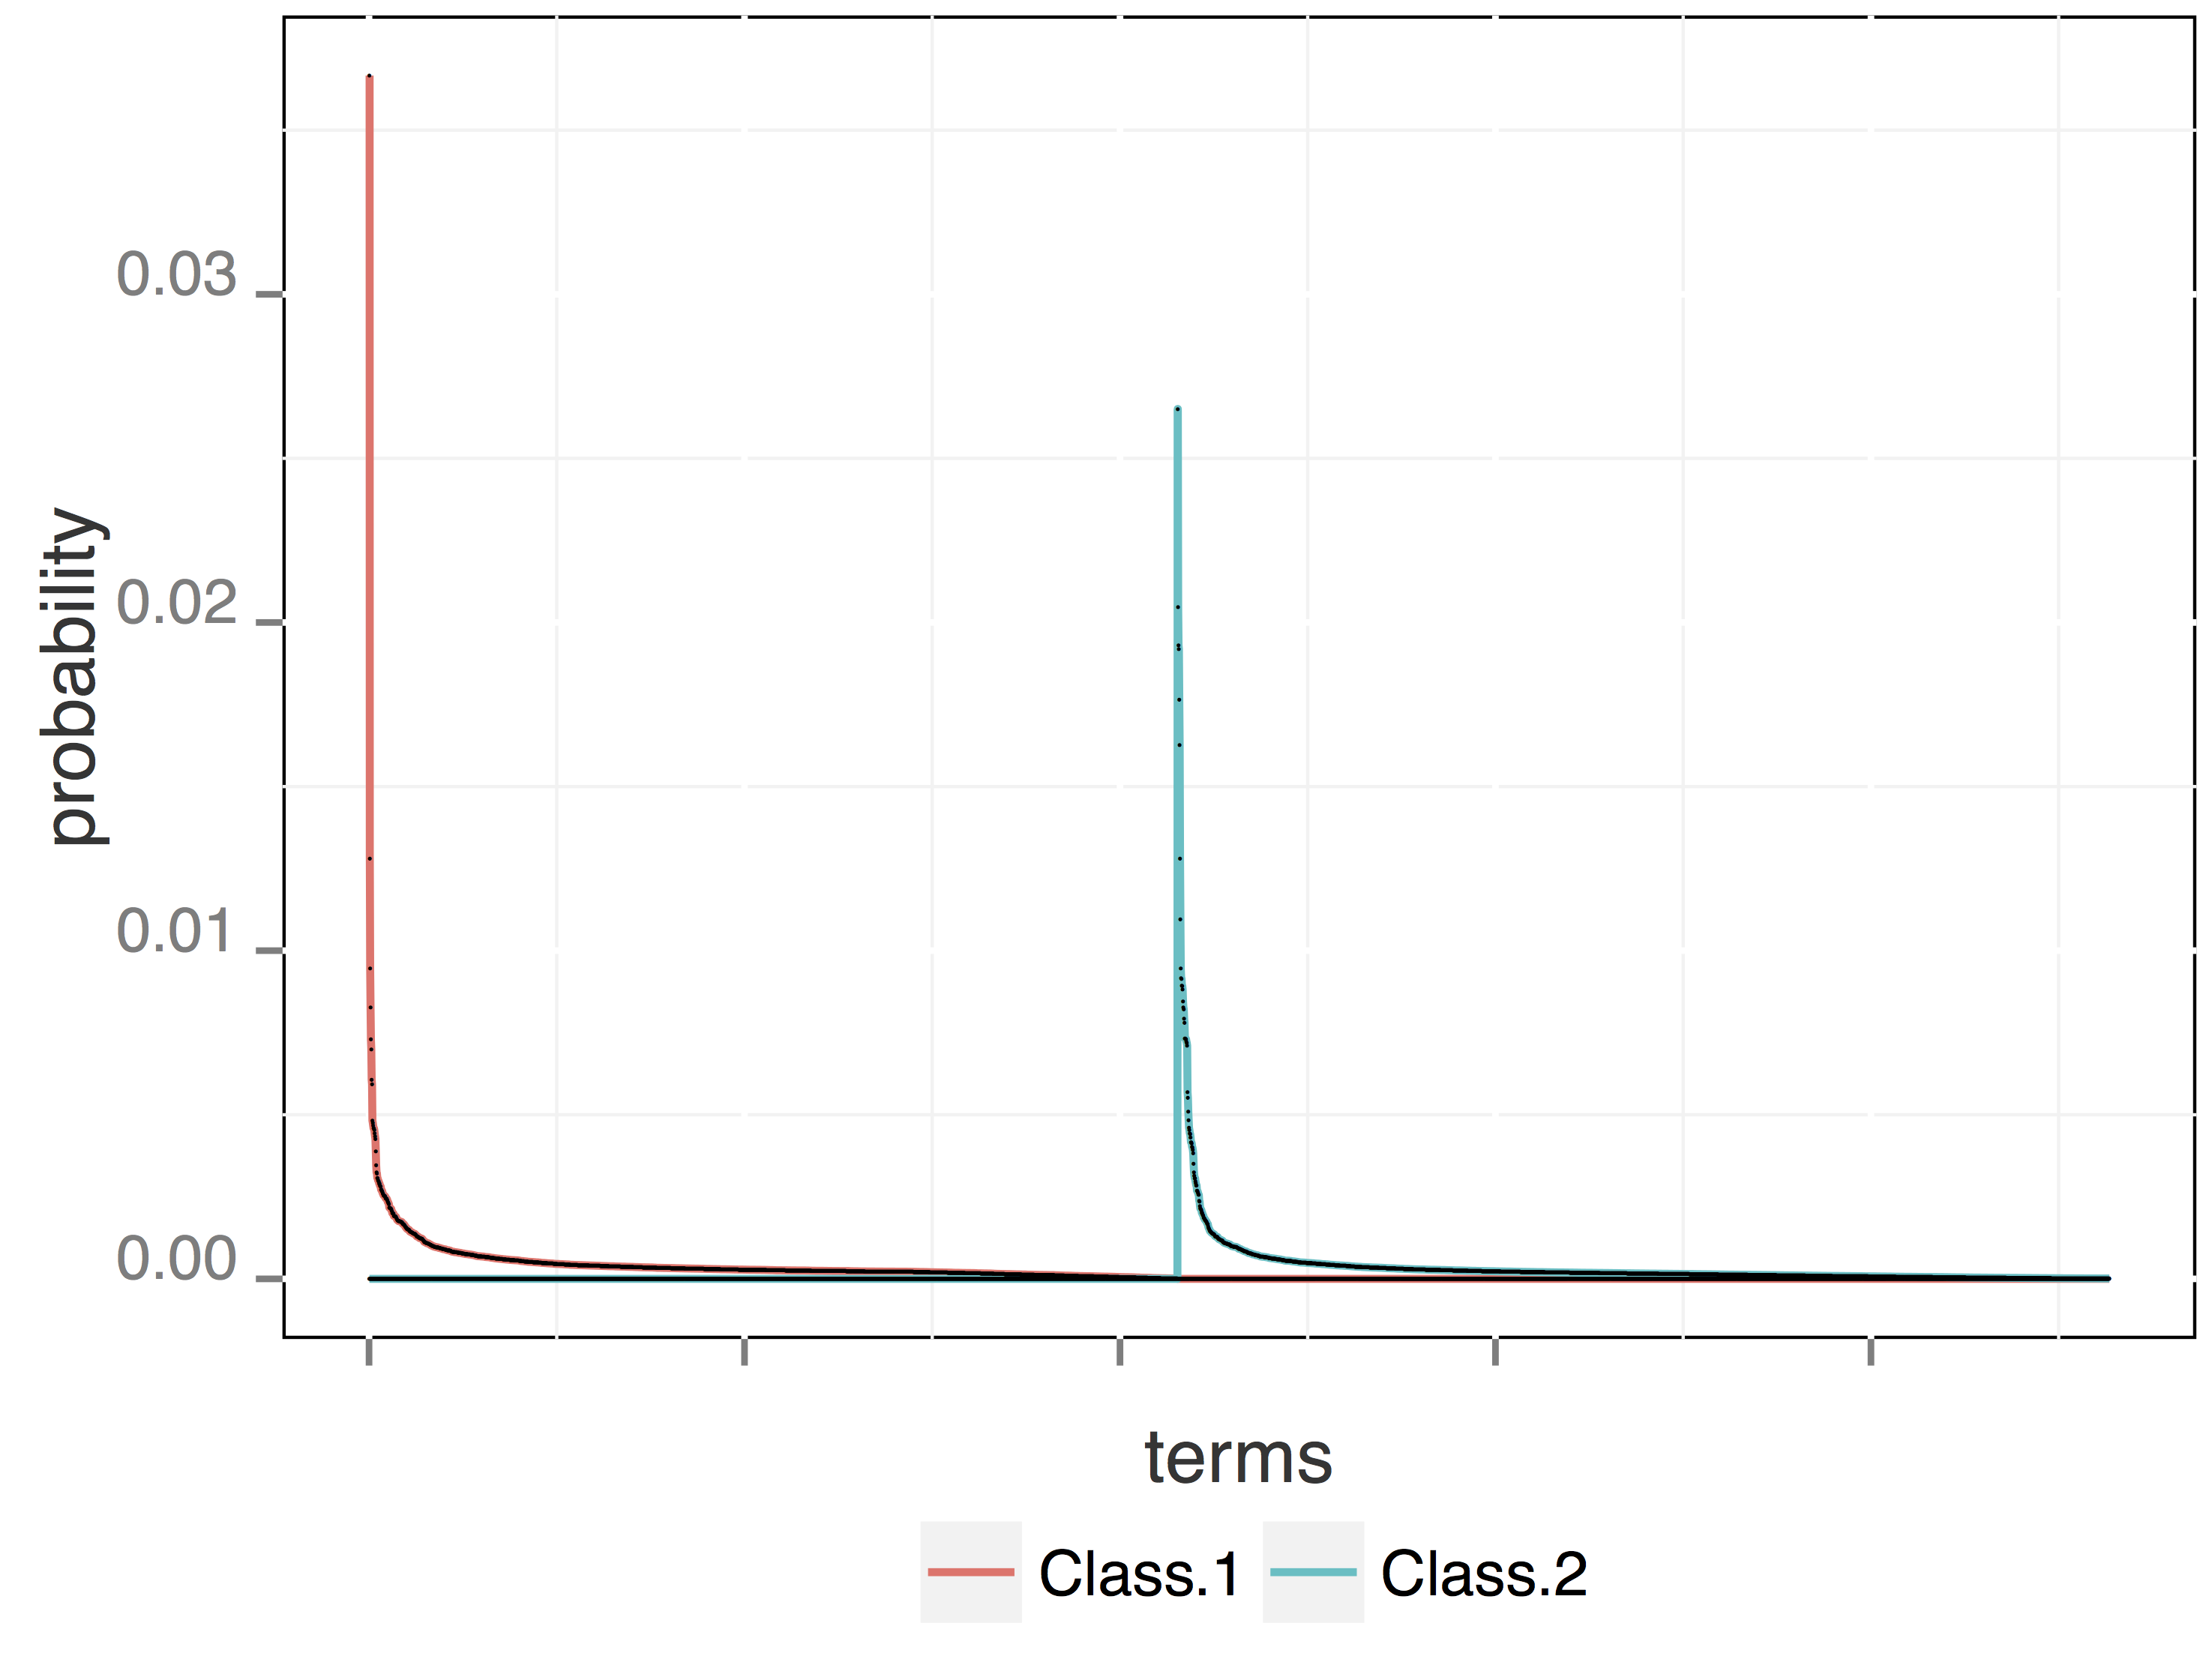
\includegraphics[width=\linewidth]{02-part-01/chapter-03/figs_and_tables/img_example-swlm.png}
\caption{\label{fig:sep-swlm} \scriptsize{A well-separable representation of data}}
\end{subfigure}
\caption{\label{fig:sep_rep} Probability distribution over terms for data in two different classes, (entities in the statues layer of the parliament), sorted based on the term weights in one of the classes.}
% }
\end{figure}
Separation in the data or feature space is a favorable property that not only helps to improve for ranking or classification algorithms but also brings out characteristic features for human inspection.
Figures~\ref{fig:sep-slm} and ~\ref{fig:sep-swlm} illustrate two different ways of modeling two entities in the status layer of the parliamentary hierarchy, i.e., government and opposition. 
Each model is a probability distribution over terms (language model) based on the speeches given by all the members in the corresponding status. In each figure, we sort the terms based on their weights in one of the models and plot the other in the same order. 
%
As can be seen, although distributions over terms in Figure~\ref{fig:sep-slm} for two classes are different, they do not suggest highly separable representations for classes. However, estimated language models in Figure~\ref{fig:sep-swlm} provide highly separable distributions over terms for two classes, identifying the characteristic terms that uniquely represent each class, and can be directly interpreted.  
 
Besides effectiveness and intractability, two\:-\:dimensional separability in the representation of hierarchical entities leads to robust models. This is due to the fact that these representations only capture solid features that remain valid even as the structure of hierarchy changes.
As an example of the importance of robust representations in evolving hierarchies, assume we would learn a representation for the ``US president'' over the current data. This is obvious that we need to distinguish the role in office from the person who is the current president; otherwise the learn representation would not be valid after the next election.  If we can separate the model of the function from the model of the person fulfilling it, for example by abstracting over several presidents, that would in principle be robust over time.

\subsection{Detailed Research Questions}
We break down our main research question in this chapter into three concrete research questions:
\begin{resqbox}
\begin{enumerate}
\item[\textbf{\resqname{c3.1}}] \emph{\resqcontent{c3.1}}
\item[\textbf{\resqname{c3.2}}] \emph{\resqcontent{c3.2}}
\item[\textbf{\resqname{c3.3}}] \emph{\resqcontent{c3.3}}
\end{enumerate}
\end{resqbox}
In the following sections, we will address these research questions.

\section{Separability in the Hierarchies}
\label{sec:sep}
In this section, we explore the first research question in this chapter:
\resq{c3.1}

In addition to the investigation of the separation property as a general foundational property of classification and defining a \emph{\ssp}, we discuss the two\:-\:dimensional separation property of hierarchical classification.

\subsection{Separation Property}
Separability is a highly desirable property for constructing and operating autonomous information systems \citep{Lewis:1995}, and especially classifiers. 
Here, we present a step by step argument which shows that based on the classification principles, having better separability in the feature space leads to better accuracy in the classification results.

%Reasoning steps:
% 0) principles:
Based on the \emph{Probability Ranking Principle (PRP)} presented by \citet{Robertson:1977}, \citet{Lewis:1995} has formulated a variant of PRP for binary classification:

\begin{displayquote}
\emph{For a given set of items presented to a binary classification system, there exists a classification of the items such that the probability of class membership for all items assigned to the class is greater than or equal to the probability of class membership for all items not assigned to the class, and the classification has optimal expected effectiveness.}
\end{displayquote}

Since in many applications, autonomous systems need to decide how to classify an individual item in the absence of entire items set, Lewis has extended the PRP to the \emph{Probability Threshold Principle (PTP)}:

\begin{displayquote}
\emph{For a given effectiveness measure,
there exists a threshold $p$, $0<p<1$, such that for any set of items, if all and only those items with probability of class membership greater than $p$ are assigned to the class, the expected effectiveness of the classification will be the best possible for that set of items.}
\end{displayquote}

PTP, in fact, discusses optimizing the effectiveness of classifiers by making items separable regarding their probability of class membership, which is a discussion on ``separability in the score space''. Based on PTP, optimizing a threshold for separating items is a theoretically trivial task; however, there are practical difficulties. 

% 1) Difficult to achieve the optimum threshold in practice (why?):
The main difficulty refers to the fact that retrieval models are not necessarily capable of measuring actual probabilities of relevance for documents \citep{Arampatzis:2001}, so they do not guarantee to generate a set of scores from which the optimum cutoff can be inferred. 
% 2) Emerging research to deal with this difficulty (analyzing score distributions of rel/irrel):
In this regard, a great deal of work has been done on analyzing the score distribution over relevant and non-relevant documents to utilize this information for finding the appropriate threshold between relevant and non-relevant documents \citep{Kanoulas:2009,Arampatzis:2009,Arampatzis:2001}. 
% 3) separability in scores distributions makes threshold finding easier -> separation property is desirable in score space!
%
It is a clear fact that the more the score distributions of relevant and non-relevant documents are separable, the easier it is to determine the optimum threshold. 
So, obtaining the \emph{separation property} in the scores distributions of relevant and non-relevant documents is one of the key focus areas for retrieval models.

% 4) separability of scores is directly related to the score generating function. But changing score generation functions to generate separable scores are complex -> instead: we can serve score functions with separable terms distribution -> then, since term dist. is a direct sign of relevancy, based on PRP, score functions are supposed to generate separable scores.
There are two ways to obtain separability in the scores distributions.  We could address the complex underlying process of score generation and investigate ranking functions that yield a separable score distribution, as in the score distributional approaches \citep{Arampatzis:2001}.  Alternatively, we can investigate ways to provide existing scoring functions with a highly separable representation of the data. 
That is, the ``term distribution'' directly provides information about the ``probability of relevance'' \citep{Crestani:1998} and if there are separable distributions over $terms$ of relevant and non-relevant documents, a scoring function satisfying PRP will generate scores that separate the classes of relevant and non-relevant documents. 
% 6)So, separation property in feature space is favorable -> Done!
Thus, a \emph{separation property} on feature distribution for representing the data is a favorable property, which follows better accuracy of classifiers' decisions.

In this chapter, we investigate the role of separation in the term or feature spaces, in which we introduce a formal definition for separability and formulate a principle on the effectiveness of classification based on separation property and leave a more formal treatment to future work.
 
As a formal and general definition, we can refer to the model separability as follows:

\begin{mydef}
\label{def:sep}
The model of an entity is epistemologically ``{separable}'' if, and only if, it has %possesses adequate 
unique, non\:-\:overlapping features that distinguish it from other models.
\end{mydef}

We argued that how separability in feature space leads to the separability in score space. Based on this and the given definition of the separability, we present \emph{\ssp (\acssp)}, which is a counterpart of the PTP~\citep{Lewis:1995} in the feature space:

\begin{displayquote}
\emph{For a given set of items presented to a classification system, for each class there exists at least one feature $\delta$ in the representation of items, and a threshold $\tau$, such that for any set of items, if all and only those items with $\delta > \tau$ are assigned to the class, the classification will have the optimal possible performance for that set of items in terms of a given effectiveness measure.}
\end{displayquote}

\acssp, in general, is a stronger version of PTP. In strict binary classification, if you have PTP, which holds on the whole feature space, \acssp will be satisfied, however in the multi-class case, \acssp is stronger and it implies PTP, but not the other way around.
Based on PTP, there is always an underlying probabilistic scoring function on the set of \emph{whole} features, which generates membership probabilities as the scores of items and these scores make items separable with regards to a threshold. So, the scoring function can be deemed as a mapping function which maps items to a new feature space in which the score of each item is a single feature representation of that item (membership probabilities (or scores) in PTP would be equivalent to $\delta$ in \acssp). Thus, when the \acssp holds, the PTP and PRP will also hold.  One could envision a stronger version of the \acssp in which ``all'' the features in the representations need to be non-overlapping, but the \acssp is sufficient for optimizing the effectiveness of the classifier.  The separation principle can be formally extended to hierarchical classification in a straightforward way.  In the rest of this section, we will discuss the separation property in the hierarchical classification and explain how to estimate separable representations with the aim of satisfying \acssp in order to improve the classification effectiveness.

\subsection{Horizontal and Vertical Separability}
\label{subsec:vhs}

In hierarchical text classification, there are two types of boundaries existing in the data, horizontal boundaries, and vertical boundaries. Hence, a separation property should be established in two dimensions. It means, not only separation between entities' representation in one layer is required, but also the separation between the distribution of terms in different layers is needed.

The separation between entities in the same layer is a related concept to the fundamental goal of all classifiers on the data with a flat structure, which is making the data in different classes distinguishable~\citep{Sebastiani:2002}. However, separation between entities in different layers is a concept related to difference of abstraction level and modeling data in different layers in a separable way can help the scoring procedures to figure out the meaning behind the layers and make their decisions less affected by the concepts of other unrelated layers, thus leading to conceptually cleaner and theoretically more accurate models.

Based on Definition~\ref{def:sep}, we formally define horizontal and vertical separability in the hierarchy as follows:
\begin{mydef}
The model of an entity in the hierarchy is ``horizontally separable'' if, and only if, it is \emph{separable} compared to other entities in the same layer, with the same abstraction level.
\end{mydef}

\begin{mydef}
The model of an entity in the hierarchy is ``vertically separable'' if, and only if, it is \emph{separable} compared to other entities in the other layers, with different abstraction levels.
\end{mydef}

To formalize these concepts, consider we have a simple three layers hierarchy of text documents with ``IsA'' relations, where the individual documents take place in the lowest layer, and each node in the middle layer determines a category, representing a group of documents, i.e., its children, and the supernode on the top of the hierarchy deemed to represent all the documents in all the groups in the hierarchy. 
%
There is a key point in this hierarchy to which we will refer for estimating models for the hierarchical entities: ``each node in the hierarchy is a general representation of its descendants''.

First assume that the goal is to estimate a language model representing category $c$, as one of the entities in the middle layer of the hierarchy, and we need the estimated model possessing \emph{horizontal separability}. 
To estimate a horizontally separable model of a category, which represents the category in a way that it is distinguishable from other categories in the middle layer, the key strategy is to eliminate terms that are common across all the categories (overlapping features) and preserve only the discriminating ones.

To do so, we consider there is a general model that captures all the \emph{common} terms of all the categories in the middle layer, $\theta_c^{g}$.  Also we assume that the standard language model of $c$, i.e the model estimated  from concatenation of all the documents in $c$ using MLE, $\theta_{c}$, is drawn from the mixture of the \emph{latent horizontally separable model}, $\theta_{c}^{hs}$, and general model that represents shared terms of all categories, i.e. $\theta_c^{g}$:
\begin{equation}
p(t|\theta_{c})  =  \lambda p(t|\theta_{c}^{hs}) + (1-\lambda) p(t|\theta_c^g),
\end{equation}
%
where $\lambda$ is the mixture coefficient.
Regarding the meaning of the relations between nodes in the hierarchy, top node in the hierarchy is supposed to be a general representation of all categories. On the other hand $\theta_c^{g}$ supposed to be a model capturing general features of all the categories in the middle layer. Thus, we can approximate $\theta_c^{g}$ with the estimated model of the top node in the hierarchy, $\theta_{all}$:
\begin{equation}
 p(t|\theta_c) \approx \lambda p(t|\theta_{c}^{hs}) + (1-\lambda) p(t|\theta_{all}).
 \label{mixture}
\end{equation}

We estimate $\theta_{all}$ using MLE as follows:
\begin{equation}
p(t|\theta_{all}) = \frac{tf(t,all)}{\sum_{t'} tf(t',all)} = \frac{\sum_{c \in all}{\sum_{d \in c}{tf(t,d)}}}{{\sum_{c \in all}{\sum_{d \in c}{\sum_{t' \in d}{tf(t',d)}}}}},
\label{eq:cmodel}
\end{equation}
where $tf(t,d)$ indicates the frequency of term $t$ in document $d$ and $\theta_{all}$ is in fact collection language model. 

Now, the goal is to extract $\theta_{c}^{hs}$. With regard to the generative models, when a term $t$ is generated using the mixture model in Equation~\ref{mixture}, first a model is chosen based on $\lambda$ and then the term is sampled using the chosen model.  The log-likelihood function for generating the whole category $c$ is:
\begin{equation}
\log p(t|\theta_{c}^{hs}) = \sum_{t \in c} tf(t,c) \log \big(\lambda p(t|\theta_{c}^{hs}) + (1-\lambda) p(t|\theta_{all})\big),
\end{equation}
where $tf(t,c)$ is the frequency of occurrence of term $t$ in category $c$. 
%Setting the parameter $\alpha$ to a fixed value and 
With the goal of maximizing this likelihood function, the maximum likelihood estimation of $p(c|\theta_{c}^{hs})$ can be computed using the Expectation-Maximization (EM) algorithm by iterating over the following steps:
\\
\textbf{E-step:}
\begin{equation}
e_t = tf(t|c).\frac{\lambda p(t|\theta_{c}^{hs})}{\lambda p(x|\theta_{c}^{hs}) + (1-\lambda) p(x|\theta_{all})}
\label{EM-E},
\end{equation}
\textbf{M-step:}
\begin{equation}
p(x|\theta_{c}^{hs}) = \frac{e_t}{\sum_{t' \in \mathcal{V}} e_t'}, \mathrm{~i.e.~normalizing~the~model},
\label{EM-M}
\end{equation}
where $\mathcal{V}$ is the set of all terms with non-zero probability in $\theta_c$. In Equation~\ref{EM-E}, $\theta_c$ is the maximum likelihood estimation of category $c$: $p(t|\theta_{c}) = \nicefrac{\sum_{d \in c}c(t,d)}{\sum_{d \in c}{\sum_{t' \in d} c(t',d)}}$ and $\theta_{c}^{hs}$ represents the horizontally separable model, which in the first iteration it is initialized by the maximum likelihood estimation, similar to $\theta_c$. 

Considering the above process, a horizontally separable model is a model which is \textbf{specified} by taking out general features that have a high probability in ``all'' categories or let's say collection language model, which is similar to the concept of the parsimonious language model, introduced by~\citet{Hiemstra:2004}.

Now assume that we want to extract a language model possessing \emph{vertical separability} for the category $c$, i.e., a model that makes this category distinguishable from entities both in the lower layer (each individual document) and the top layer (collection of all documents).
%
In the procedure of making the model horizontally separable, we argued that we can reduce the problem to removing terms representing the top node, which results in a model that is separable from the top node in the upper layer. This means that we are already half-way towards making a model vertically separable; thus, the model only requires to be separable from its descendant entities in the lower layer.  
Back to the meaning of the ``IsA'' relations in the hierarchy, the model of each node is a general representation of all its descendants. So making the model of a category separable from its descendant documents means to remove terms that describe each individual documents, but not all of them. We call these terms, document specific terms.

For each category $c$, we assume there is a  model, $\theta_d^{s}$, that captures document specific terms, i.e. terms from documents in that category that are good indicators for individual documents but not supported by all of them. Also we assume that the standard language model of $c$, $\theta_{c}$, is drawn from the mixture of the \emph{latent vertically separable model}, $\theta_{c}^{vs}$, and $\theta_d^{s}$: 
\begin{eqnarray}
p(t|\theta_{c}) & = & \lambda p(t|\theta_{c}^{vs}) + (1-\lambda) p(t|\theta_d^s)
\end{eqnarray}
where $\lambda$ is the mixing coefficient. 
We estimate $\theta_d^s$ using the following equation:
\begin{equation}
p(t|\theta_d^s)  \xleftarrow{normalized} 
\sum_{d_i\in c} 
\bigg(
p(t|\theta_{d_i}) \prod_{\substack{d_j\in c \\ j \neq i}} (1-p(t|\theta_{d_j}))
\bigg),
\label{eq:smodel}
\end{equation}
where $p(t|\theta_{d_i}) = \nicefrac{c(t,d_i)}{\sum_{t' \in d_i} c(t',d_i)}$. This equation assigns a high probability to a term if it has high probability in one of the document models, but not others, marginalizing over all the document models.  This way, the higher the probability is, the more specific the term will be. 
Now, the goal is to extract the $\theta_{c}^{vs}$. An EM algorithm, similar to Equations~\ref{EM-E} and~\ref{EM-M} can be applied for estimating $\theta_{c}^{vs}$ by removing the effect of $\theta_d^s$ from $\theta_{c}$.

Considering the above process, a vertically separable model is a model which is \textbf{generalized} by taking out specific terms that have a high probability in one of the descendant documents, but not others.  

\subsection{Two\:-\:Dimensional Separability}
In order to have fully separable models in hierarchical classification, they should own two\:-\:dimensional separation property. We define two\:-\:dimensional separability as follows:
\begin{mydef}
The model of an entity in the hierarchy is ``two\:-\:dimensionally separable'' if, and only if, it is both horizontally and vertically separable at the same time.
\end{mydef}

Intuitively, if a model of an entity is two\:-\:dimensionally separable, it should capture \emph{all}, and \emph{only}, the essential features of the entity taking its relative position in the hierarchy into consideration.  In the next section, we will discuss how to estimate two\:-\:dimensional separable models for entities in the hierarchies with more than three layers.


\section{\HSWLMs}
\label{sec:hswlm}
In this section, we address the second research question of this chapter:
\resq{c3.2}

We introduce \Hswlms (\achswlm) which is an extension of \SWLM that is explained in chapter~\ref{chap:2} tailored to textual hierarchical entities. \achswlm is, in fact, a particular arrangement of multiple passes of the procedures of making the models of hierarchical entities vertically and horizontally separable, as they are explained in Section~\ref{subsec:vhs}.
%
We use the idea of parsimonious language models \cite{Hiemstra:2004} to parsimonize the representation of an entity by down-weighting terms that do not reflect the significant features of that entity, with regards to its position in the hierarchy.   
In the parsimonious language model, given a raw probabilistic estimation, the goal is to re-estimate the distribution so that non-essential parameters of the raw estimation are down-weighted if they are well explained in a given background distribution. 
The proposed approach for estimating \hswlm iteratively reestimates the standard language models of entities to minimize their overlap by discarding non\:-\:essential terms from them. 

In the original parsimonious language model~\citep{Hiemstra:2004}, the background model is explained by the estimation of the \emph{collection model}, i.e., the model representing all the entities, similar to Equation~\ref{eq:cmodel}.  
However, with respect to the hierarchical structure, and our goal in \achswlm for making the models of entities separable from each other, we need to use the parsimonization technique in two different directions: 1) given ancestors of an entity, and 2) given its descendants. Hence, besides parsimonizing given a single parent entity in the upper layers, as the background model, we need to be able to do parsimonization given multiple descendants in the lower layers. 
\begin{figure}[!t]
\centering
\begin{algorithm}[H]
 \begin{algorithmic}[1]
 \Procedure{Parsimonize}{$e$,$B$}
 \ForAll{term $t$ in the vocabulary}
     \State \begin{small}$P(t|\theta_B) \xleftarrow{normalized} \sum_{b_i\in B} \bigg(P(t|\theta_{b_i}) \prod_{\substack{b_j\in B \\ j \neq i}} (1-P(t|\theta_{b_j}))\bigg)$ \end{small}
     \Repeat
         \State \begin{small}E-Step: $P[t\in \mathcal{V}] \gets P(t|\theta_e).\frac{\alpha P(t|\tilde{\theta}_e)}{\alpha P(t|\tilde{\theta}_e) + (1-\alpha) P(t|\theta_B)}$ \end{small}
          \State \begin{small}M-Step: $P(t|\tilde{\theta}_e) \gets \frac{ P[t \in \mathcal{V}]}{\sum_{t' \in \mathcal{V}} P[t' \in \mathcal{V}]}$ \end{small}
     \Until{$\tilde{\theta_t}$ becomes stable}
 \EndFor
 \EndProcedure
 \end{algorithmic}
 \caption{Modified Model Parsimonization}
\end{algorithm}
\caption{Pseudo-code for procedure of modified model parsimonization.}
\end{figure}
Algorithm~\ref{alg:model_parsimonization} presents pseudo-code of the Expectation-Maximization algorithm which is employed in the modified model parsimonization procedure. 
In the equation in line 3 of the pseudo-code in Algorithm~\ref{alg:model_parsimonization}, $B$ is the set of background entities\:---\:either one or multiple, and $\theta_{b_i}$ demonstrates the model of each background entity, $b_i$, which is estimated using MLE. As can be seen, in case of having a single ancestor node as the background model,  this equation will be equal to Equation~\ref{eq:cmodel} and in case of having multiple descendants as the background models, it results same as Equation~\ref{eq:smodel}. 
In this procedure, in general, in the E-step, the probabilities of terms are adjusted repeatedly, and in the M-step, adjusted probability of terms are normalized to form a distribution. 
Another change in the modified version of model parsimonization, which practically makes no difference in the final estimation, is that in the E-step, instead of using $tf(t,e)$, we employ $p(t|\theta_e)$, where $\theta_e$ is the model represents entity $e$ and initially it is estimated using MLE. This is because in the multi-layer hierarchies, there is more than one parsimonization pass for a particular entity and after the first round, we need to use the probability of terms estimated from the previous pass, not the raw information of their frequency.

\begin{figure}[!t]
\centering
\begin{algorithm}[H]
 \begin{algorithmic}[1]
 \Procedure{Estimate{\achswlm}s}{}
 \Statex ~~~~Initialization: \vspace{2pt}
 \ForAll{entity $e$ in the hierarchy}
 \State $\theta_e \gets$ standard estimation for $e$ using MLE
% \Statex ~~~~~~~~~(using Maximum Likelihood Estimation)
 \EndFor
 \Repeat
 \State \Call{Specification}{}
 \State \Call{Generalization}{} 
 \Until{models do not change significantly anymore}
 \EndProcedure
 \end{algorithmic}
 \caption{Estimating \HSWLM}
\end{algorithm}
\caption{\label{alg:hswlm}Pseudo-code for the overall procedure of estimating \achswlm.}
\end{figure}
Model parsimonization is an almost parameter free process. The only parameter is the standard smoothing parameter $\lambda$, which controls the level of parsimonization, so that the lower values of $\lambda$ result in more parsimonious models.
The iteration is repeated a fixed number of times or until the estimates do not change significantly anymore. 

The pseudo-code of the overall procedure of estimating \achswlm is presented in Algorithm~\ref{alg:hswlm}. 
Before the first round of the procedure, a standard estimation like maximum likelihood estimation is used to construct the initial model for each entity in the hierarchy. 
Then, models will be updated in an iterative process until all the estimated models of entities become stable. 
In each iteration, there are two main stages: a \emph{Specification stage} and a \emph{Generalization stage}. 
In these stages, language models of entities in the hierarchy are iteratively made ``specific,'' by taking out terms explained at higher levels, and ``general,'' by eliminating specific terms of lower layers, which results in models that are both \emph{horizontally} and \emph{vertically} separable as it is described in Section~\ref{subsec:vhs}.

\begin{figure}[!t]
\centering
\begin{algorithm}[H]
\captionsetup{labelformat=empty}
\begin{algorithmic}[1]
\Procedure{Specification}{}
\State Queue $\gets$ all entities in breadth first order
\While{Queue is not empty}
  \State $e \gets$ Queue.pop()
  \State $l \gets e$.Depth()
  \While{$l > 0$}
    \State $A \gets e$.\Call{getAncestor}{$l$}
    \State \Call{Parsimonize}{$e$,$A$}
    \State $l \gets l-1$  
  \EndWhile
\EndWhile
\EndProcedure
\end{algorithmic}
\captionof{algorithm}{Specification Stage}
\end{algorithm}
\caption{\label{alg:specification_stage}Procedure of Specification. $e$. Function \Call{getAncestor}{$l$} gives the ancestor of entity $e$ with $l$ edges distance from it. Function \textsc{Parsimonize}($e$,$B$)  parsimonizes $\theta_e$ given background models in $B$}
\end{figure}
In the specification stage, the goal is to eliminate the general terms of the language model of each entity so that the resulted language model demonstrates the entity's specific properties.  
To do so, the parsimonization method is used to parsimonize the language model of an entity given its ancestors, from the root of the hierarchy to its direct parent, as the background estimations. 
%
The order in the hierarchy is of crucial importance here. 
When a language model of an ancestor is considered as the background language model, it should demonstrate the ``specific'' properties of that ancestor. Due to this fact, it is important that before considering the language model of an entity as the background estimation, it has already passed the specification stage, and we have to move top-down.
Pseudo\:-\:code of the recursive procedure of specification of entities' models in the hierarchy is depicted in Algorithm~\ref{alg:specification_stage}.

% \begin{figure}[!t]
% \centering
\begin{algorithm}[t!]
% \captionsetup{labelformat=empty}
\begin{algorithmic}[1]
\Procedure{Generalization}{}
\State Stack $\gets$ all entities in breadth first order
\While{Stack is not empty}
  \State $e \gets$ Stack.pop()
  \State $l \gets e$.Height()
  \While{$l > 0$}
    \State $D \gets e$.\Call{getDecedents}{$l$}
    \State \Call{Parsimonize}{$e$,$D$}
    \State $l \gets l-1$  
  \EndWhile
\EndWhile
\EndProcedure
\algrule
 \LineComment{Function \Call{getDecedents}{$l$} gives all the decedents of entity $e$ with $l$ edges distance from it. Function \textsc{Parsimonize}($e$,$B$)  parsimonizes $\theta_e$ given background models in $B$ (Algorithm~\ref{alg:model_parsimonization}).}
\end{algorithmic}
% \captionof{algorithm}{Generalization Stage}
\caption{\label{alg:generalization_stage}Procedure of Generalization.}
\end{algorithm}
% \caption{\label{alg:generalization_stage}Procedure of Generalization. $e$. Function \Call{getDecedents}{$l$} gives all the decedents of entity $e$ with $l$ edges distance from it. Function \textsc{Parsimonize}($e$,$B$)  parsimonizes $\theta_e$ given background models in $B$.}
% \end{figure}
In the generalization stage, the goal is to refine language models by removing terms which do not address the concepts in the level of abstraction of the entity's layer.
To do so, again parsimonization is exploited but given descendants, which leads to the elimination of specific terms. 
Here also, before considering the model of an entity as the background estimation, it should be already passed the generalization stage, so generalization moves bottom up.
Algorithm~\ref{alg:generalization_stage} presents the pseudo\:-\:code for the recursive procedure of generalization of entities' language models in the hierarchy. 
In the generalization step, the background models of descendants are supposed to be specific enough to show their extremely specific properties. Hence, generalization stages must be applied on the output models of specification stages: specification should precede generalization, as shown in Algorithm~\ref{alg:hswlm} before.

\section{\achswlm for Hierarchical Classification}
Two-dimensional separability as the main properties of \achswlm makes the learned representations of the entities in the hierarchy less sensitive to the structural changes for instance when the hierarchy evolves over time. Here in this section, we address our last research question of this chapter:
\resq{c3.3}

Before evaluating the transferability of two-dimensionaly separable representations over time, we intrinsically study the separability of the representations learned by \achswlm. We use parliamentary data as one of the interesting collections with hierarchically structured data that can evolve over time. The structure of the parliamentary hierarchy has been shown in Figure~\ref{fig:ParHierarchy}.  First, we introduce the collection we have used, and then we analyze the quality of \achswlm on providing horizontal and vertical separability over the hierarchy. 

\subsection{Data Collection}
We use the Dutch parliamentary data which forms a hierarchical structure that can evolve over time. The data are collected and annotated as the part of
\emph{Political\-Mashup} project \citep{url:politicalmashup} to make semantically enriched parliamentary proceedings available as open data \citep{marx:2010}.

As a brief background, the Dutch parliament is a bicameral parliament which consists of the Senate and the house of representatives. The house of representatives is the main chamber of parliament, where discussion of proposed legislation and review of the government's actions takes place.  The Dutch parliamentary system is a multi-party system, requiring a coalition of parties to form the government~\citep{deswaan73}.

\begin{figure*}[!t]
\centering
\makebox[\linewidth][c]{
\resizebox{\linewidth}{!}{%
\tikzset{
every tree node/.style={align=center,anchor=north}
edge from parent/.style={very thick},
%edge from parent/.style=
%{draw, edge from parent path={(\tikzparentnode.south)
%-- +(0,-8pt)
%-| (\tikzchildnode)}},
blank/.style={draw=none}}
\begin{tikzpicture}[level distance = 30pt]
\fontsize{7}{8}\selectfont{
\matrix (magic) [ampersand replacement=\&]
{
\node{\Tree
    [.All  \edge[blank]; 
    [.Status  \edge[blank];
    [.Party \edge[blank]; 
    [.Mem\# ]]]]};
\&
\node{
    \Tree 
    [.\small{Parliament(2006-2010)}
        [.Government 
            [.$CDA$  $47$ ]
            [.$PvdA$  $37$ ]
            [.$CU$  $6$ ]
        ]
        [.Opposition 
            [.$VVD$  $24$ ]
            [.$PVV$  $10$ ]
            [.$SP$  $27$ ]
            [.$D66$  $3$ ]
            [.$GL$  $10$ ]
        ]
    ]};
\&
\node{
    \Tree 
    [.\small{Parliament(2010-2012)}
        [.Government 
            [.$VVD$  $33$ ]
            [.$CDA$  $23$ ]
        ]
        [.Oppositions
            [.$PvdA$  $32$ ]
            [.$PVV$  $22$ ]
            [.$SP$  $16$ ]
            [.$D66$  $10$ ]
            [.$CU$  $6$ ]
            [.$GL$  $12$ ]
        ]
    ]};
\&
\node{
    \Tree 
    [.\small{Parliament(2012-2014)}
        [.Government 
            [.$VVD$  $43$ ]
            [.$PvdA$  $42$ ]
        ]
        [.Opposition 
            [.$CDA$  $13$ ]
            [.$PVV$  $12$ ]
            [.$SP$  $18$ ]
            [.$D66$  $12$ ]
            [.$CU$  $5$ ]
            [.$GL$  $4$ ]
        ]
    ]};\\
};
}
\end{tikzpicture}
}
}
\caption{Composition of Dutch parliament in 3 periods. \emph{VVD}:People's Party for Freedom and democracy, \emph{PvdA}:Labour Party, \emph{CDA}:Christian Democratic Appeal, \emph{PVV}:Party for Freedom, \emph{SP}:The Socialist Party, \emph{D66}:Democrats 66, \emph{GL}:Green-Left, \emph{CU}:Christian-Union.}
\label{fig:DutchParl}
\end{figure*}
We use data from the parliament or the House of Representatives of the Netherlands.  We have chosen three interesting periods of parliament, from March 2006 to April 2014, in which eight main parties have about 95\% of seats in the parliament: People's Party for Freedom and Democracy, Labour Party, Christian Democratic Appeal, Party for Freedom, The Socialist Party, Democrats 66, Green-Left, Christian-Union.   The coalition in the first period is between a left-wing party and a centrist party, in the second period between a right-wing party and centrism party, and in the third, between a right-wing and left-wing party. Figure~\ref{fig:DutchParl} shows the hierarchical structure of the Dutch parliament in these three different periods.

In order to learn representations for parliamentary entities, first of all,  we prepare the data. In the proceedings, there are series of parliamentary speeches by different MPs following the debate structure.  We invert the data matrix so that for each speaker we collect their speeches as a single document that reflects the features of that member. Then, for representing the internal entities in the parliament's hierarchy, we first consider members as the leaf entities and then concatenate all leaf documents below internal entities as a single document which textually represents them: first over parties, and then parties into government and opposition, etc.
%
The whole corpus consists of 14.7 million terms from 240,501 speeches and contains 2.1 million unique terms. 
No stemming and no lemmatization is done on the data and also stop words, and common words are not removed in data preprocessing.  After data preparation, we estimate \acswlm\ for all entities in the hierarchy as it is explained in Section~\ref{sec:hswlm}.

%---------------------------------------
\subsection{Two-Dimensional Separability of \achswlm}
\label{subsec:achswlmep}
%---------------------------------------
Here we investigate the ability of \achswlm on providing language models for hierarchical entities that are two-dimensionally separable. 
Based on the explained procedure of estimating \achswlm, the language models of entities in the hierarchy is repeatedly updated, so that the resulting models are both \emph{horizontally} and \emph{vertically} separable in the hierarchy. To assess this fact, we estimate \achswlm on the parliamentary data and look into the separability between entities in the same layer or in different layers.

Figures~\ref{fig:HSS} and~\ref{fig:HSP} illustrate the probability distribution over terms based on the estimated \achswlm in the status and party layer respectively. We sort the probability distribution on the term weight of the first model and plot the other models in this exact order.
As can be seen in the status layer, Figures~\ref{fig:HSS}, the distributions over terms for government and opposition cover almost separated set of terms. Since in this layer these two entities are supposed to be against each other, a high level of separability can be expected. On the other hand, in the party layer, Figures \ref{fig:HSP}, it is possible that two parties share some ideological issues and consequently share some terms. So, in this layer, a complete separability of terms would not be practically possible for all the parties. Nevertheless, \achswlm provides an acceptable horizontal separability in this layer.


\begin{figure}[t]
    \centering
    \begin{subfigure}[b]{0.32\textwidth}
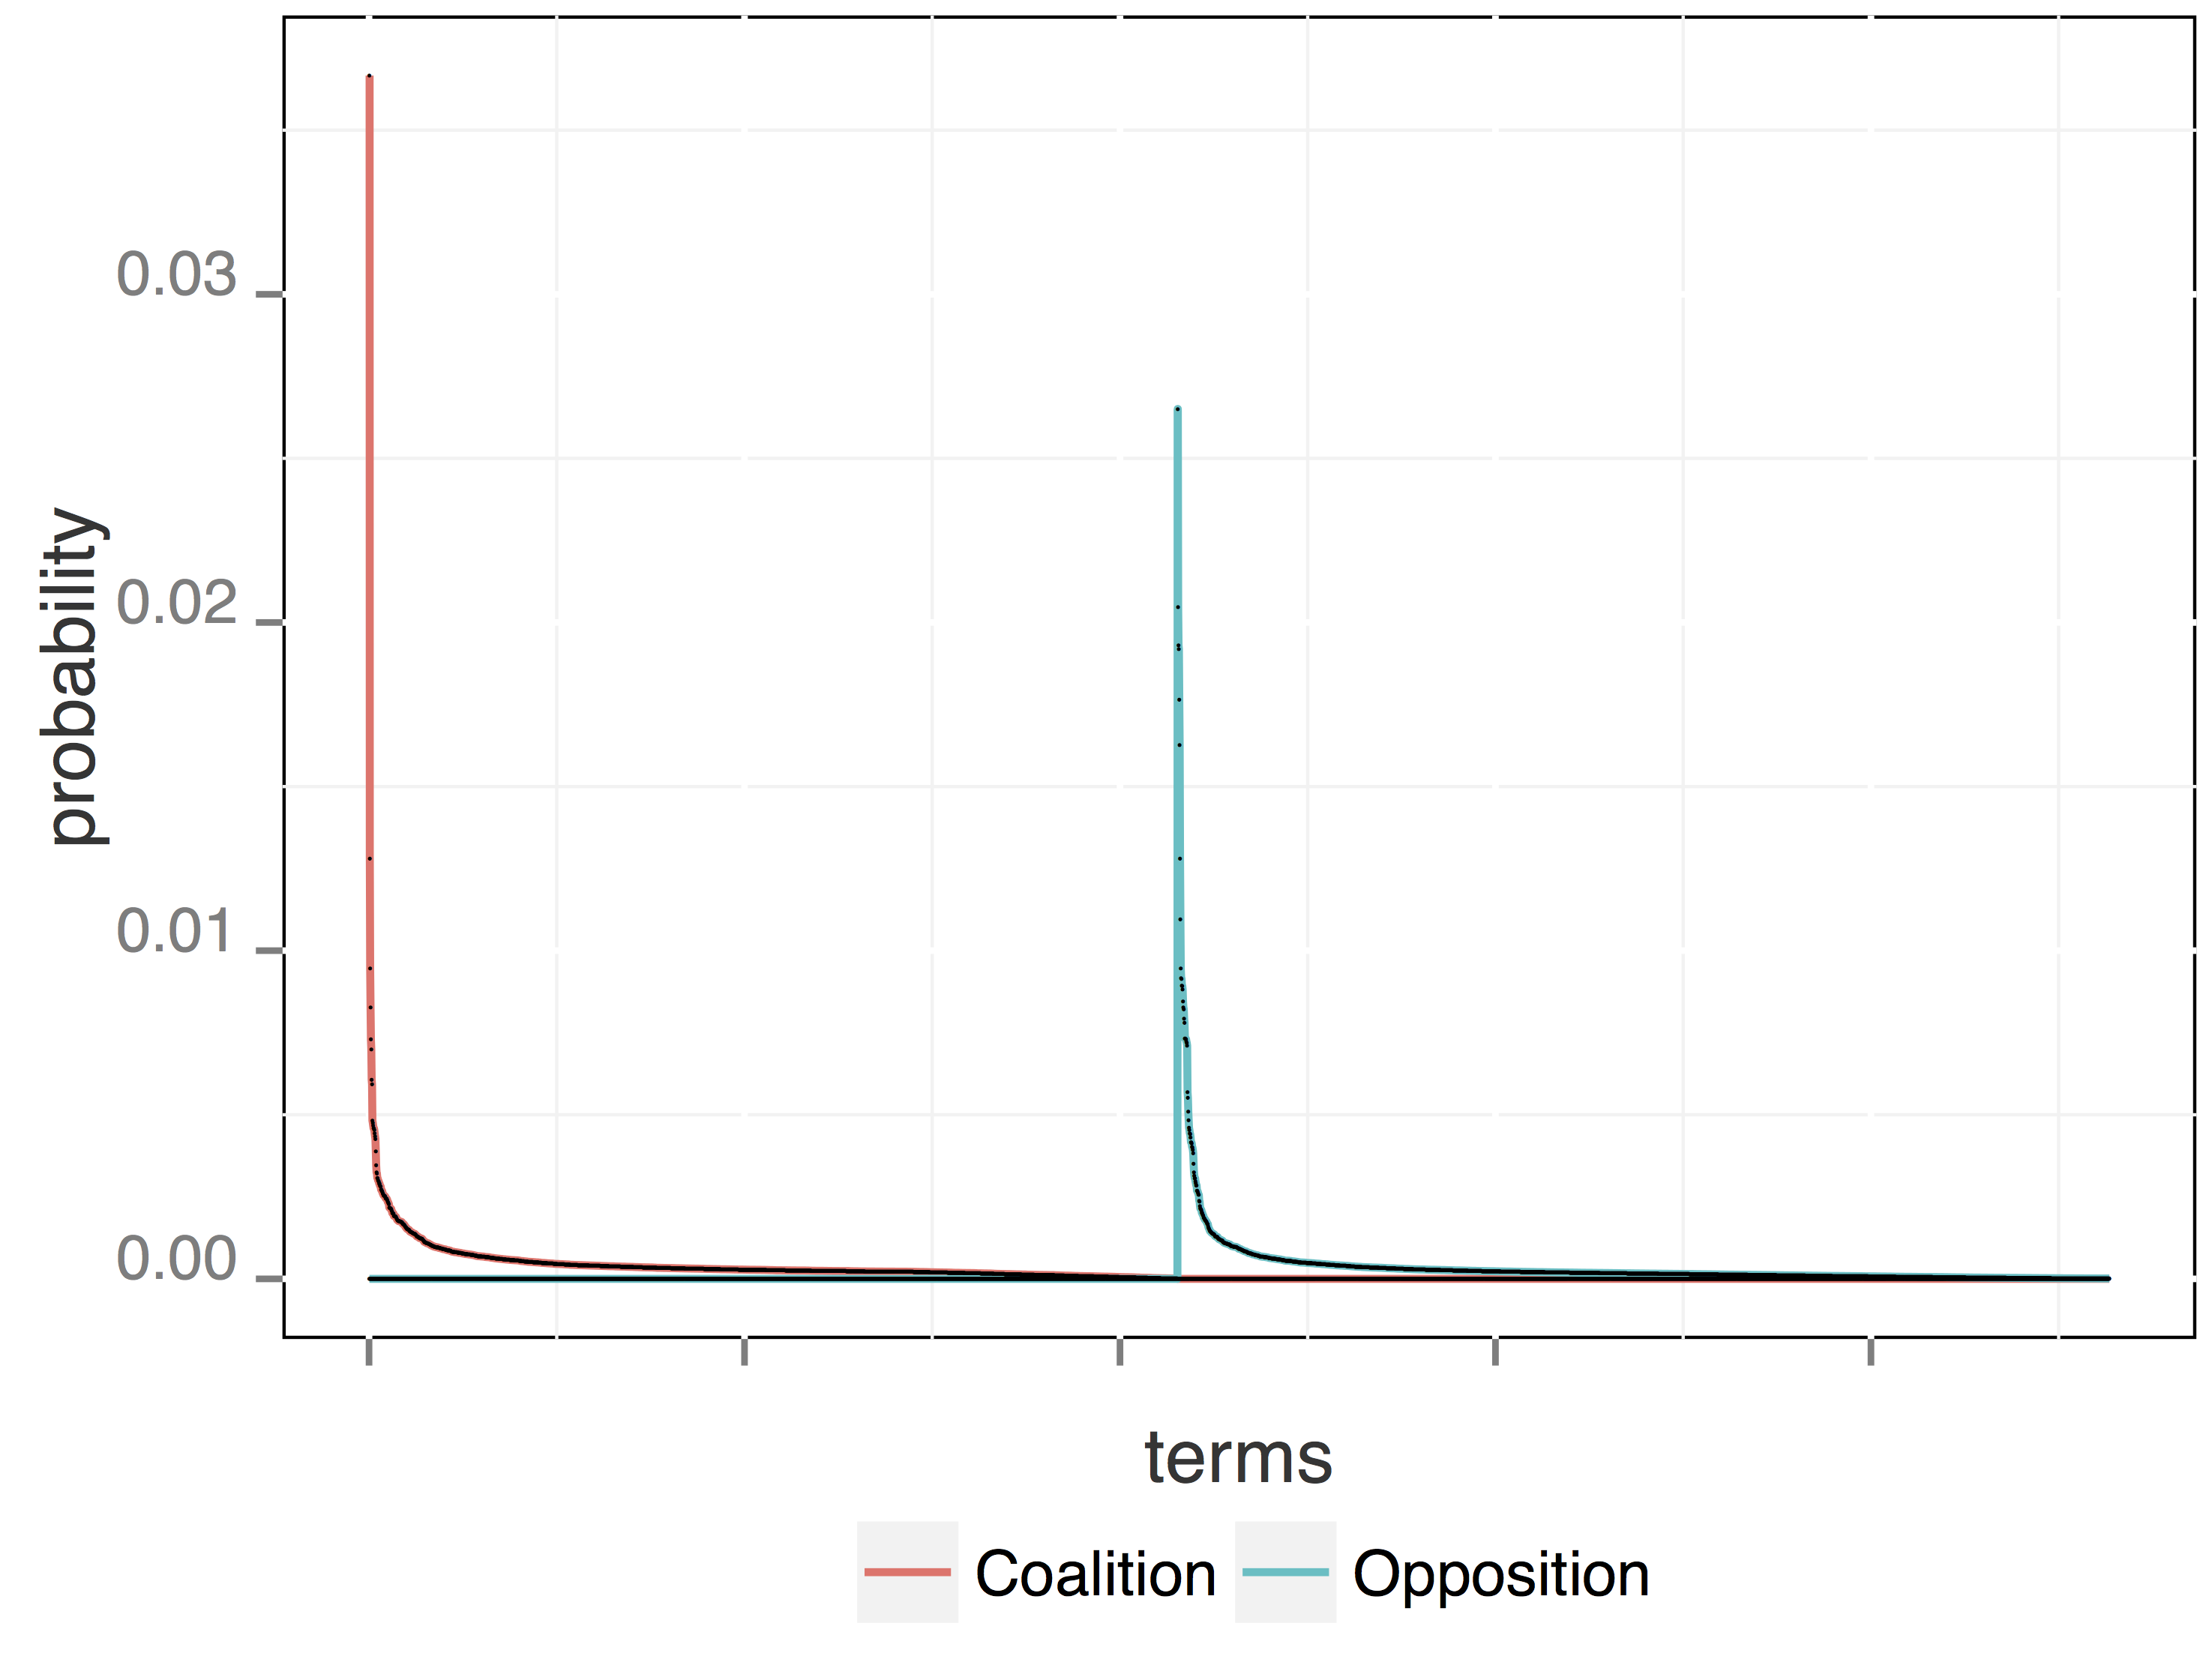
\includegraphics[width=\linewidth]{02-part-01/chapter-03/figs_and_tables/img_opo-coa.png}
\caption{\label{fig:HSS}\achswlm in the status layer}
        \end{subfigure}
        ~ 
    \begin{subfigure}[b]{0.64\textwidth}
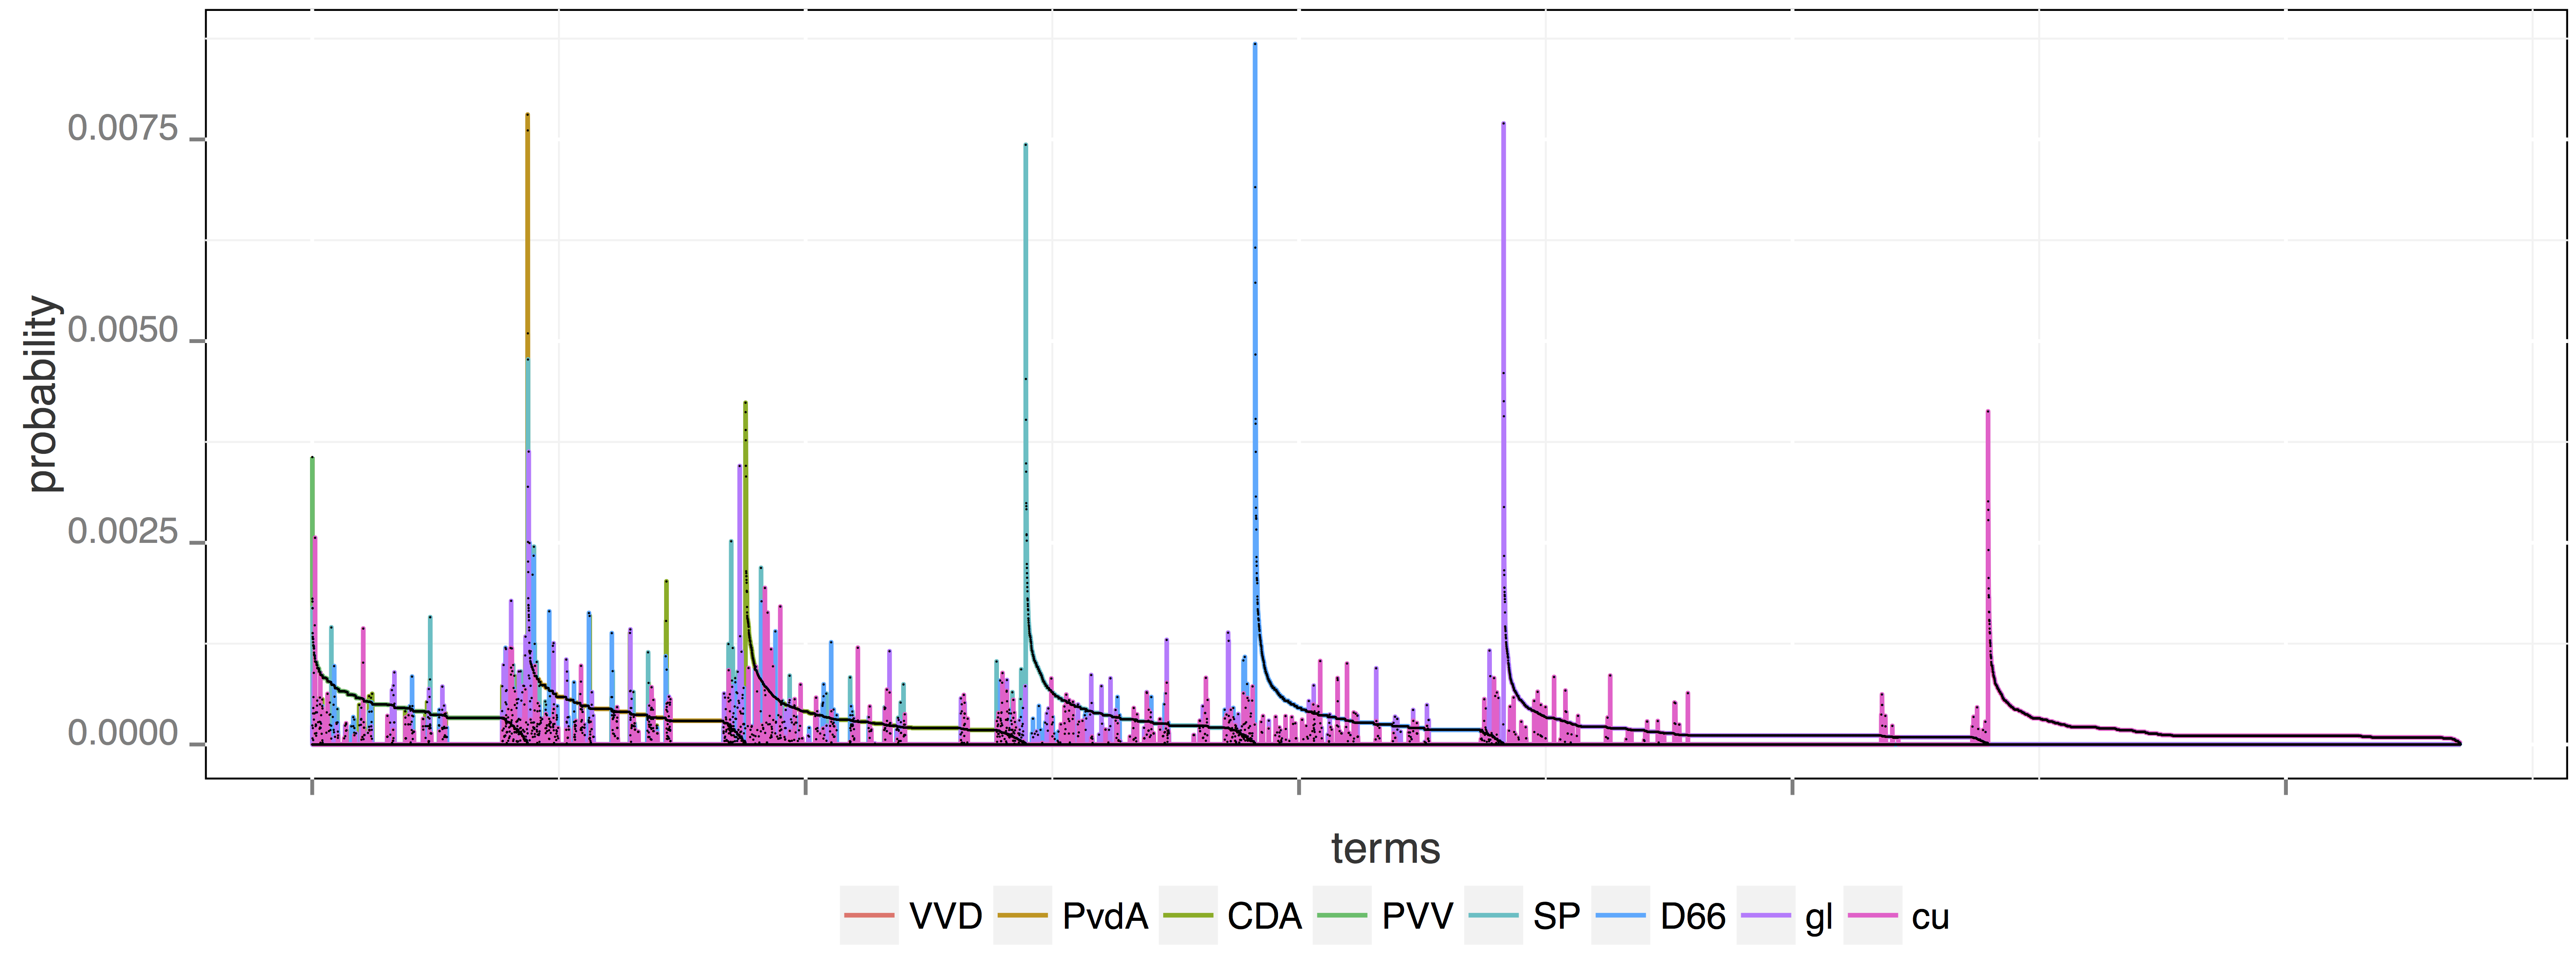
\includegraphics[width=\linewidth]{02-part-01/chapter-03/figs_and_tables/img_parties.png}
\caption{\label{fig:HSP}\achswlm in the party layer}
        \end{subfigure}
    \caption{\label{fig:HS} \emph{Horizontal Separability}: probability distribution over terms based on \hswlms in status layer and party layer.}
\end{figure}

Besides, we illustrate the horizontal separability of \achswlm of some pairs of parties. Figures \ref{fig:HSPCO}, \ref{fig:HSPOO}, and \ref{fig:HSPCC} show the separability of models of two parties in three cases, respectively: 1) different statuses, 2) both in the status of opposition, 3) both in the status of government. It can be seen that in all cases of being in the same status or different status, estimated \hswlms are separable. The interesting point is in Figure~\ref{fig:HSPCC} that presents the models of two government parties that are strongly separable. This rooted in the fact that in this period there was an unusual coalition government consisting of a right-wing and a left-wing party. So, although they have an agreement in the status layer, their model is highly separable in terms of having opposite spectrum in party layer.


\begin{figure}[!t]
        \centering
        \begin{subfigure}[b]{0.32\textwidth}
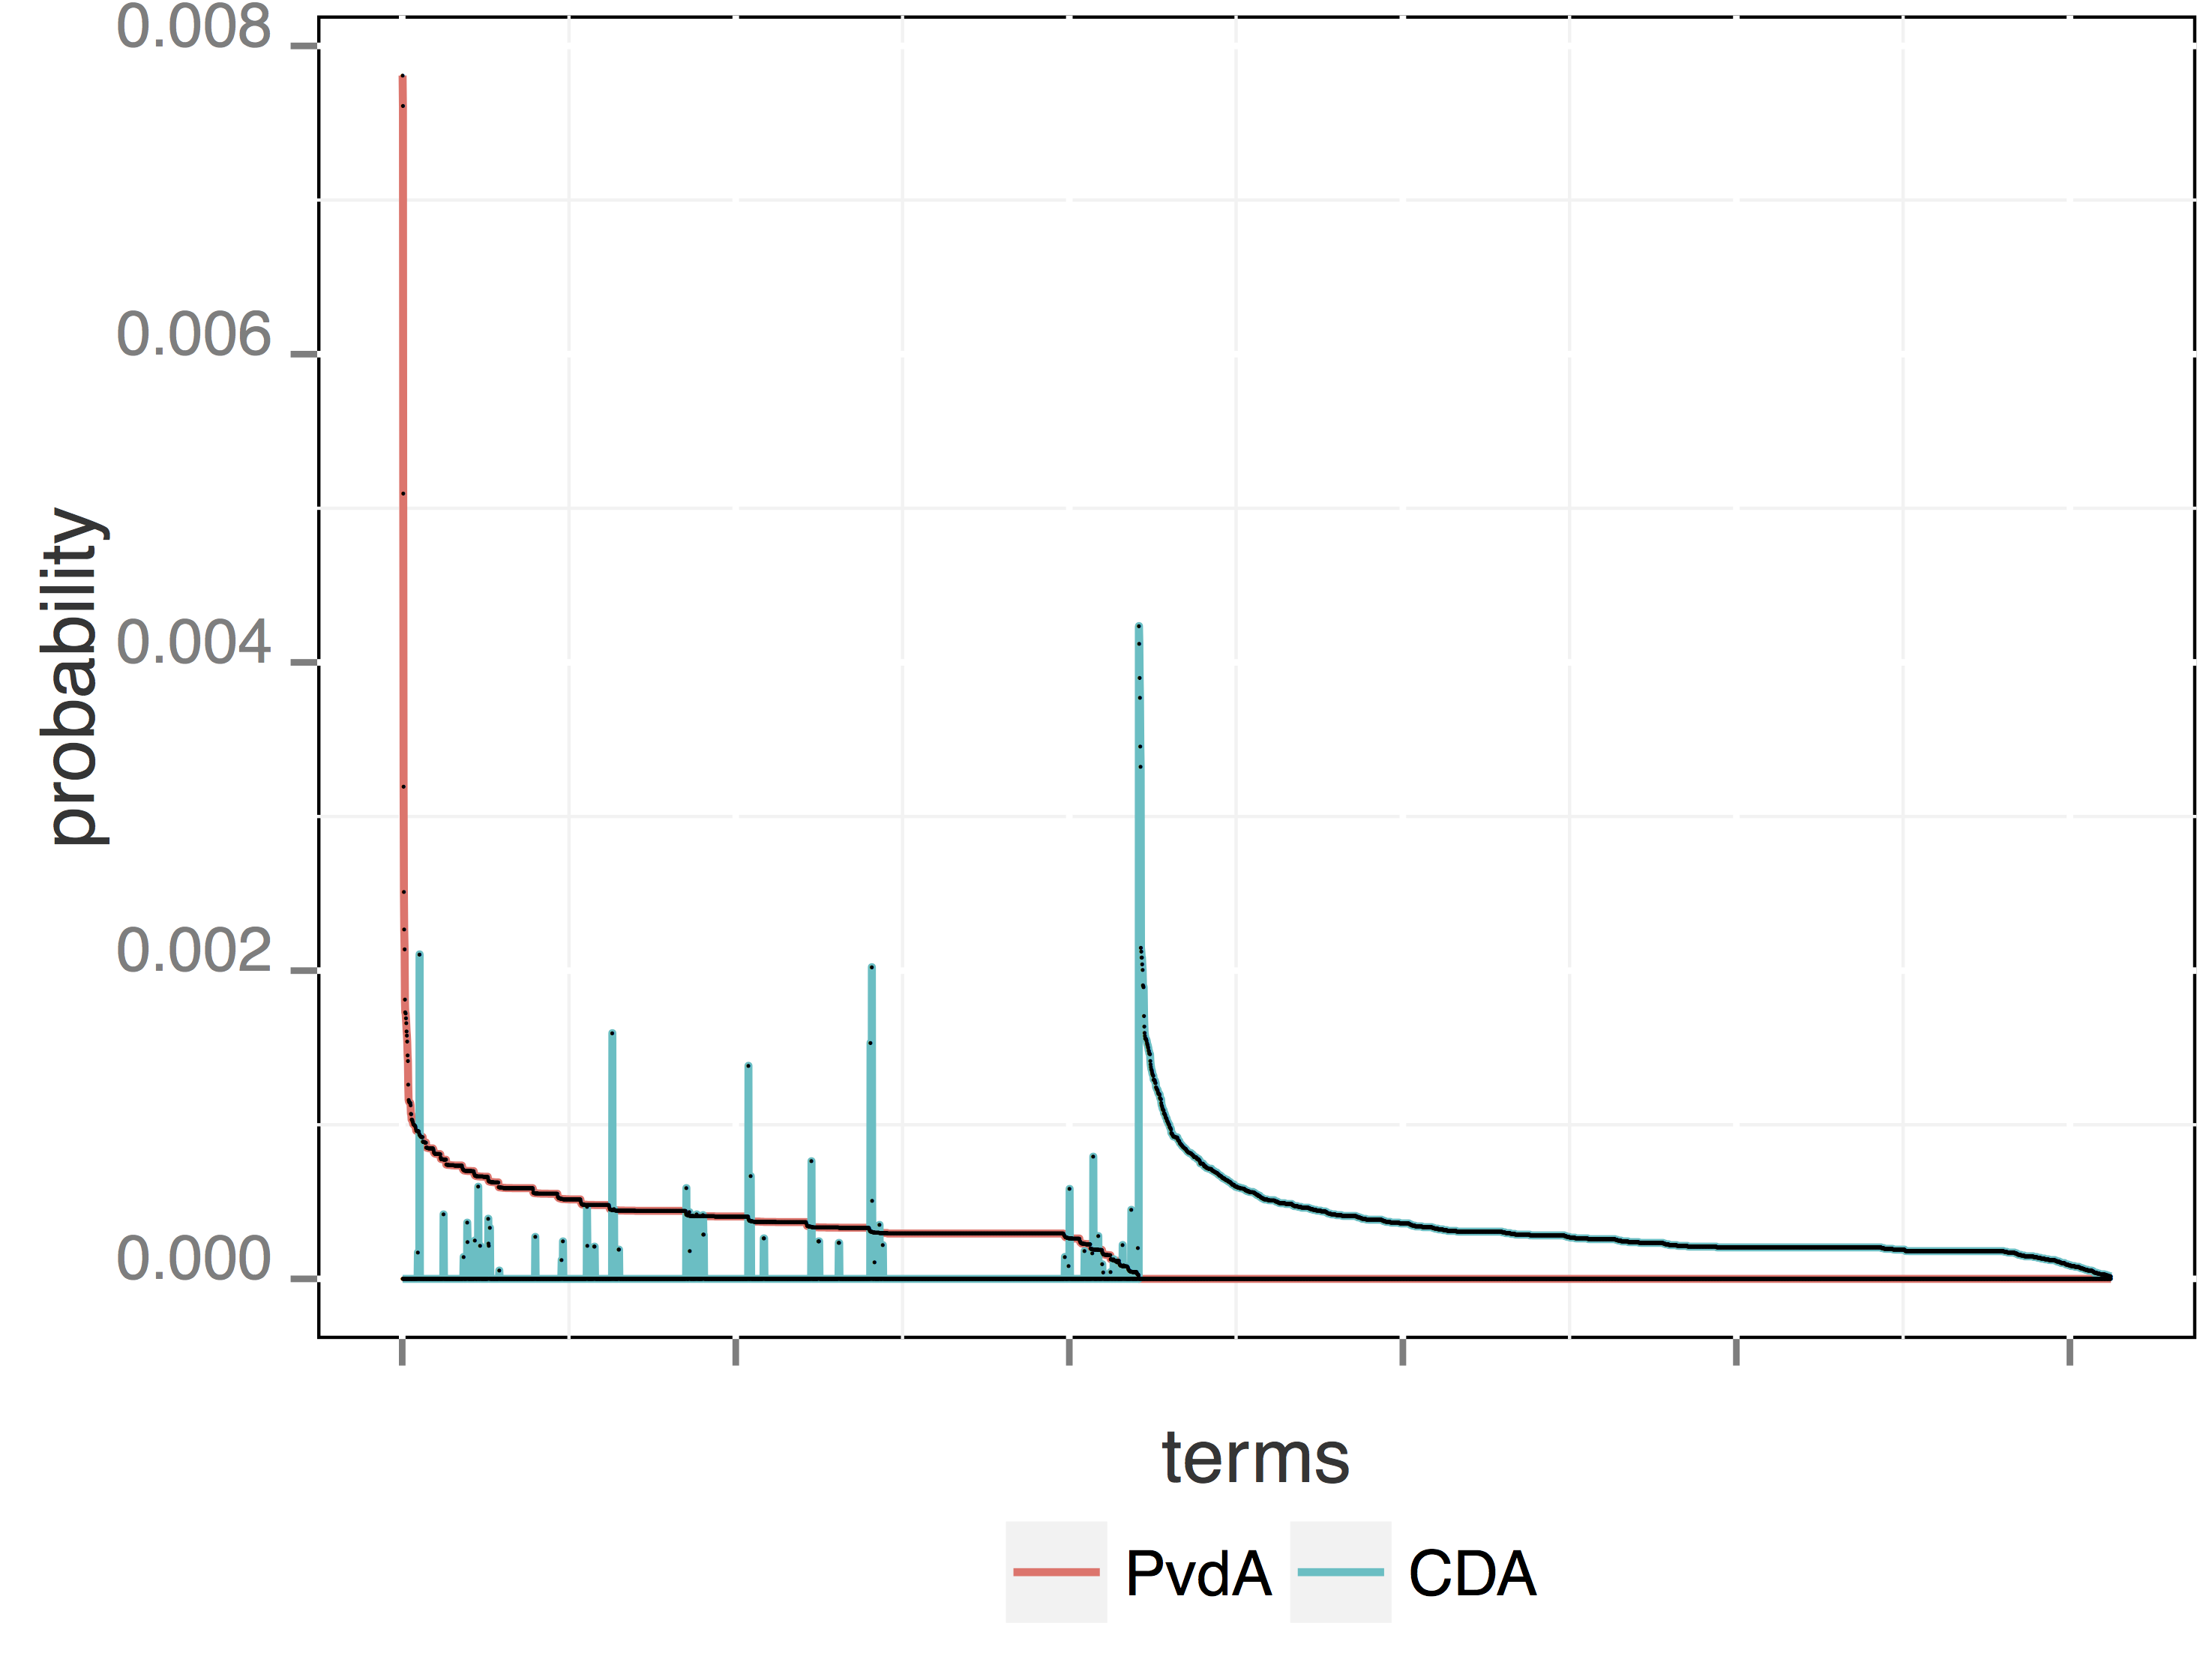
\includegraphics[width=\linewidth]{02-part-01/chapter-03/figs_and_tables/img_PvdA-CDA.png}
\caption{\label{fig:HSPCO} \achswlm of two parties in different statuses: Christian Democratic Appeal (CDA) and Labour Party (PvdA)}
        \end{subfigure}
        ~ 
        \begin{subfigure}[b]{0.32\textwidth}
\centering
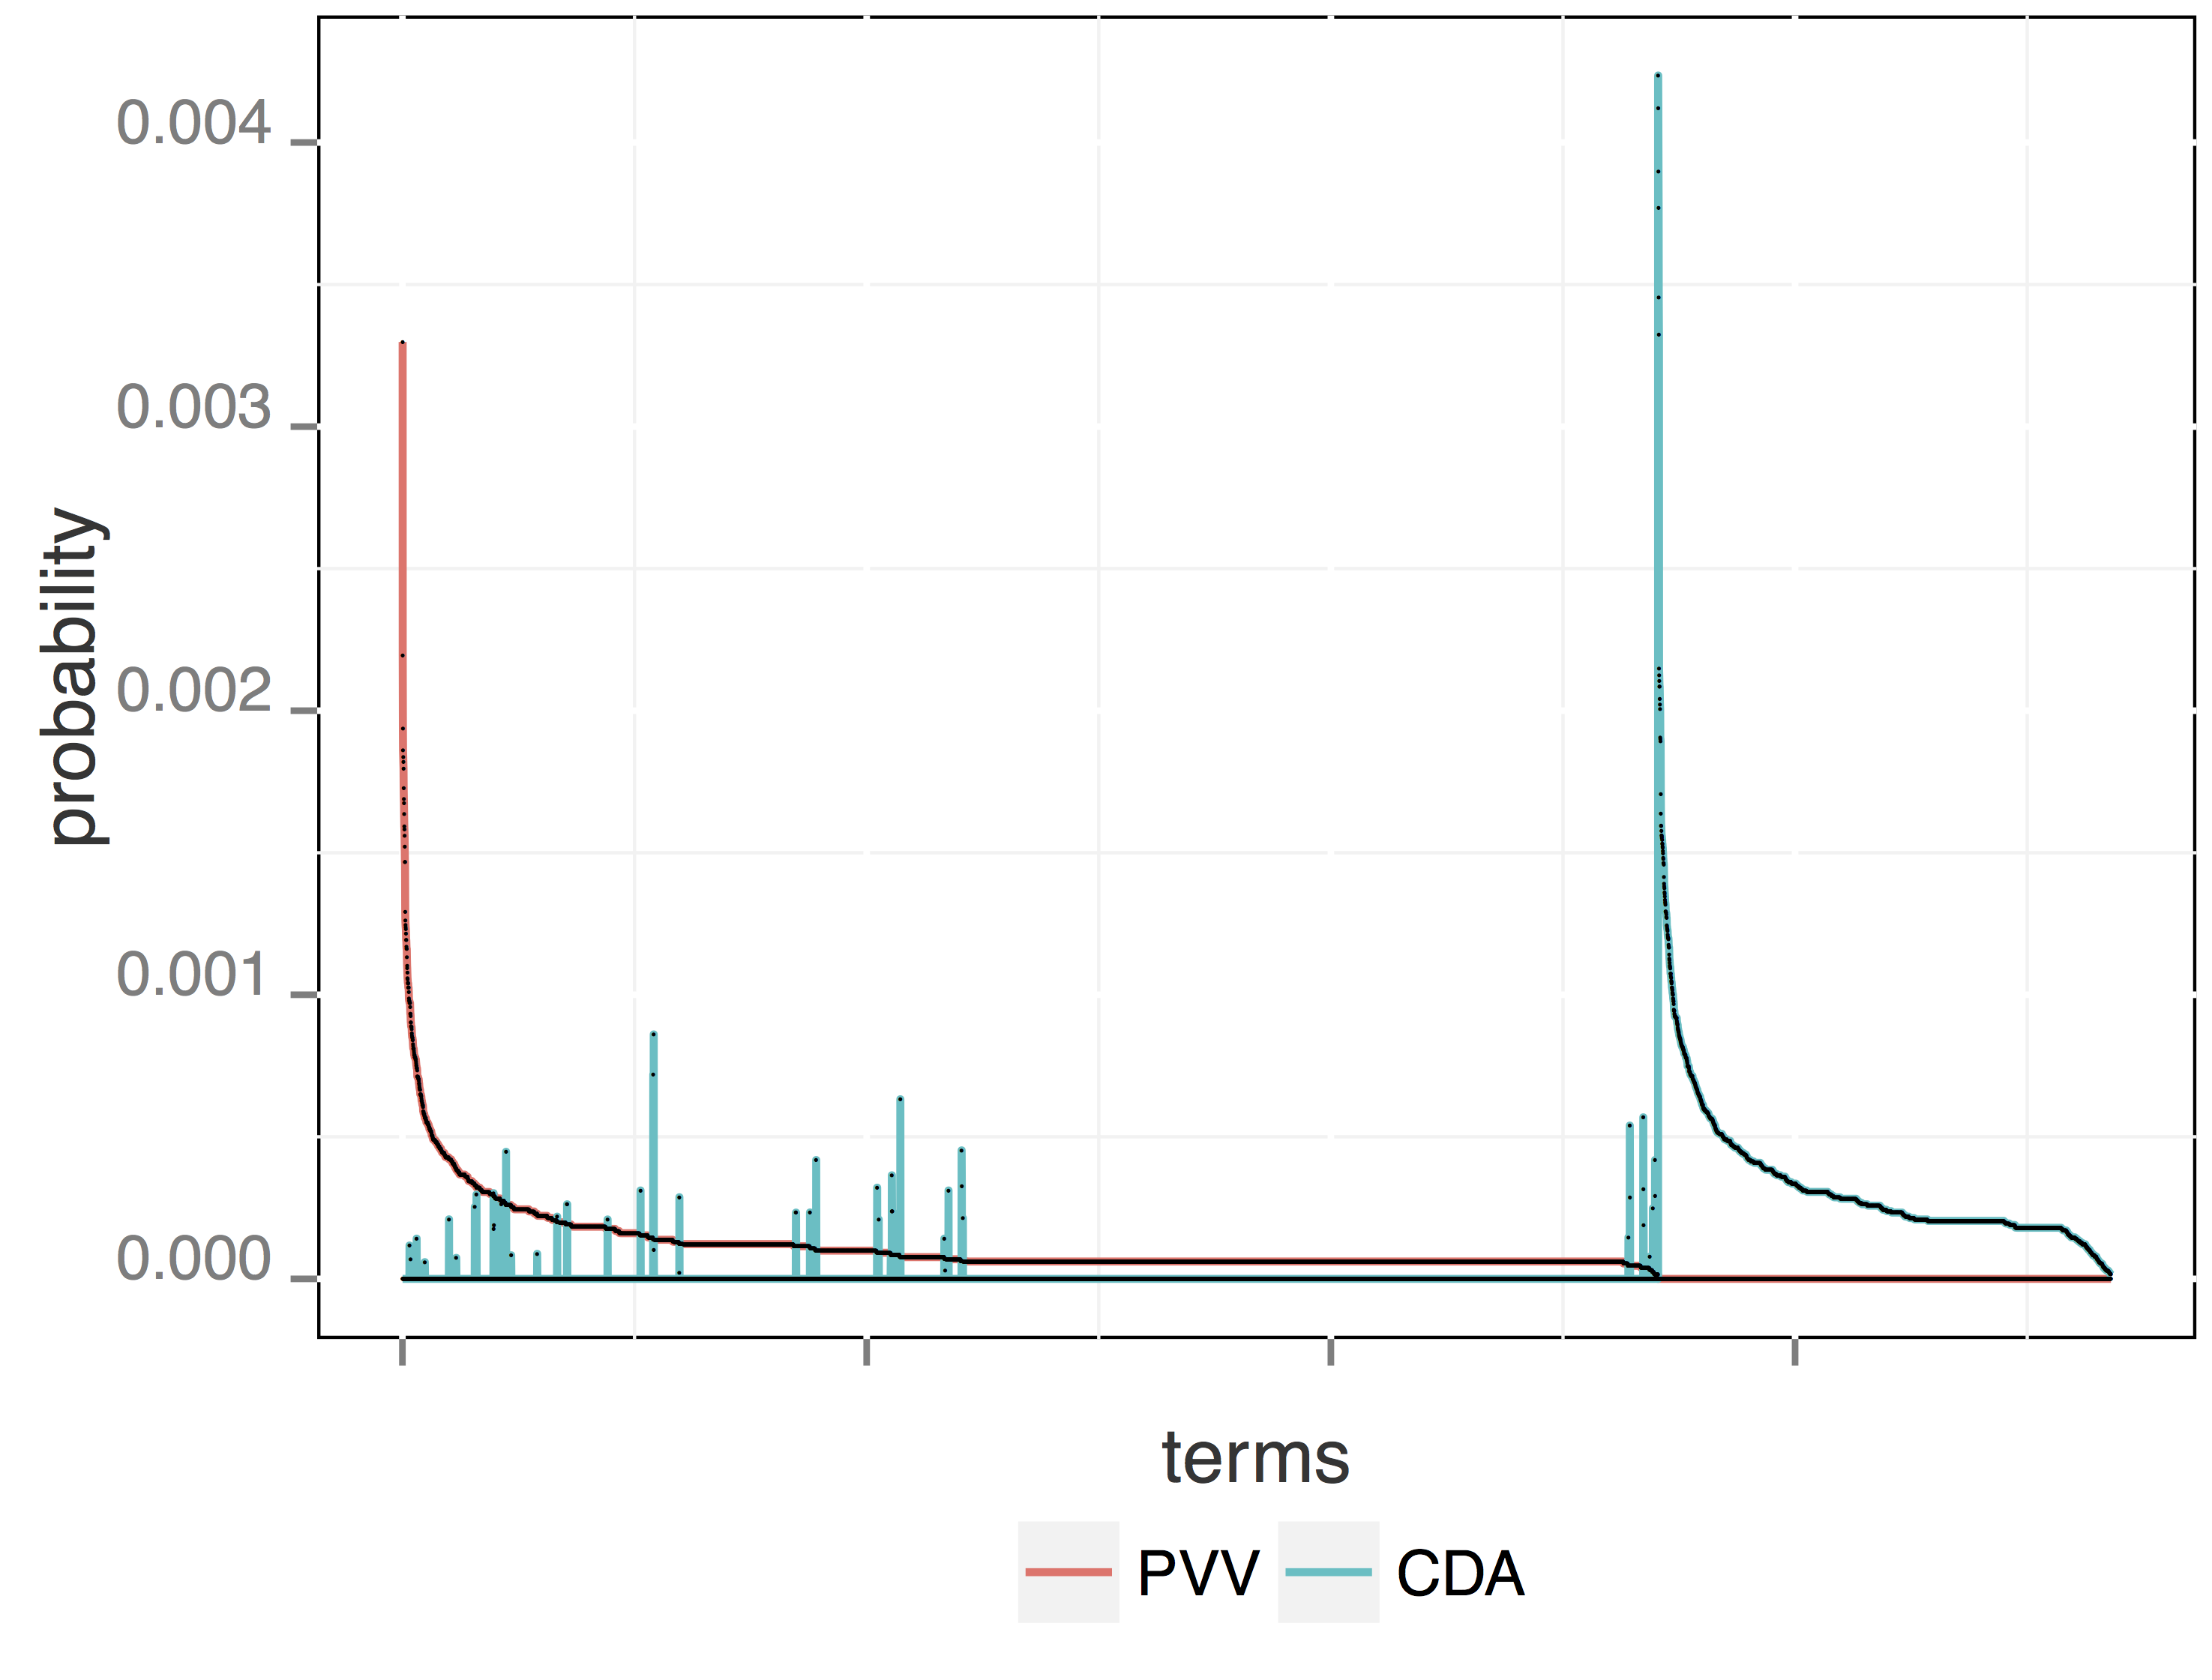
\includegraphics[width=\linewidth]{02-part-01/chapter-03/figs_and_tables/img_PVV-CDA.png}
\caption{\label{fig:HSPOO} \achswlm of two parties in opposition: Party for Freedom (PVV) and Christian Democratic Appeal (CDA)}
        \end{subfigure}
        ~ 
        \begin{subfigure}[b]{0.32\textwidth}
\centering
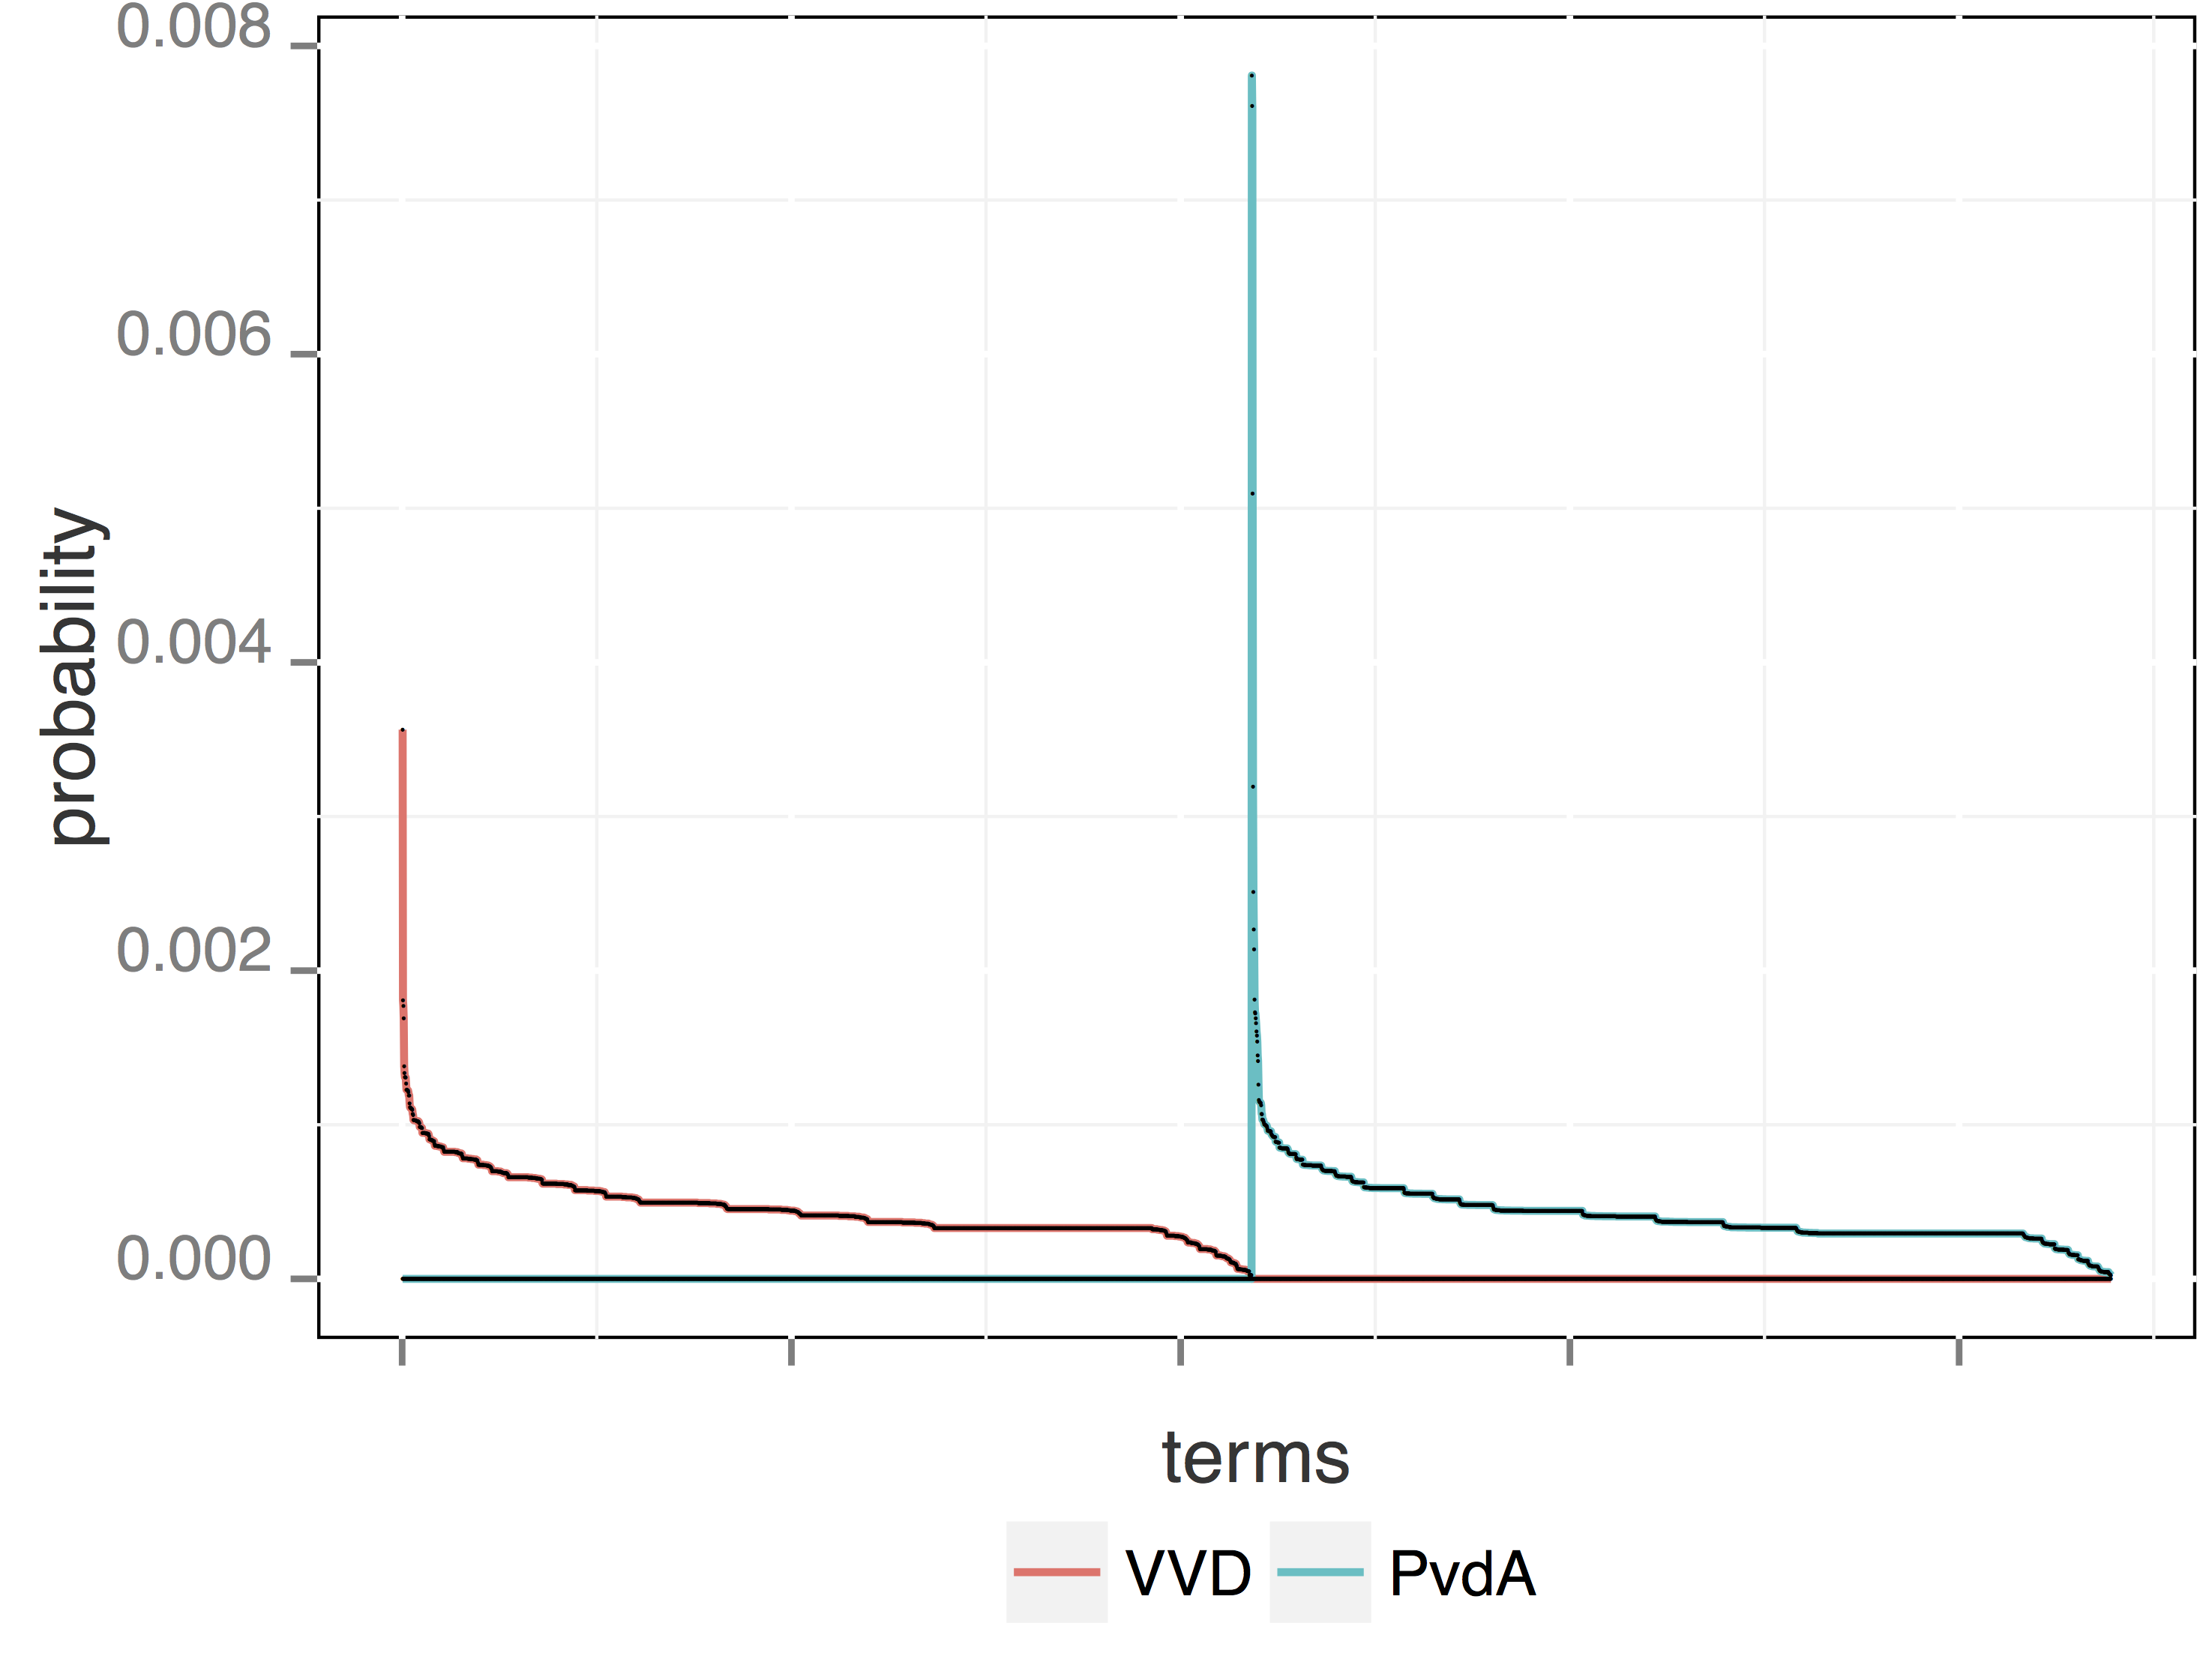
\includegraphics[width=\linewidth]{02-part-01/chapter-03/figs_and_tables/img_VVD-PvdA.png}
\caption{\label{fig:HSPCC} \achswlm of two parties in government: People's Party for Freedom (VVD) and Labour Party (PvdA)}
        \end{subfigure}
        \caption{\label{fig:HSP-pairs} \emph{Horizontal Separability}: probability distribution over terms based on \hswlms in party layer}
\end{figure}

In order to illustrate the vertical separability of \achswlm, we choose two different branches in the hierarchy: one from the leader of one of the opposition parties to the root, and the other from the leader of one of the government parties to the root. Figures \ref{fig:VSO} and \ref{fig:VSC} show probability distributions over words based on \achswlm of all entities in these two branches. They demonstrate that using \achswlm, we can decompose distribution over all terms to the highly separable distributions, each one representing the language usage related to the meaning behind the layer of the entity in the hierarchy. 

\begin{figure}[!t]
        \centering
        \begin{subfigure}[b]{0.45\textwidth}
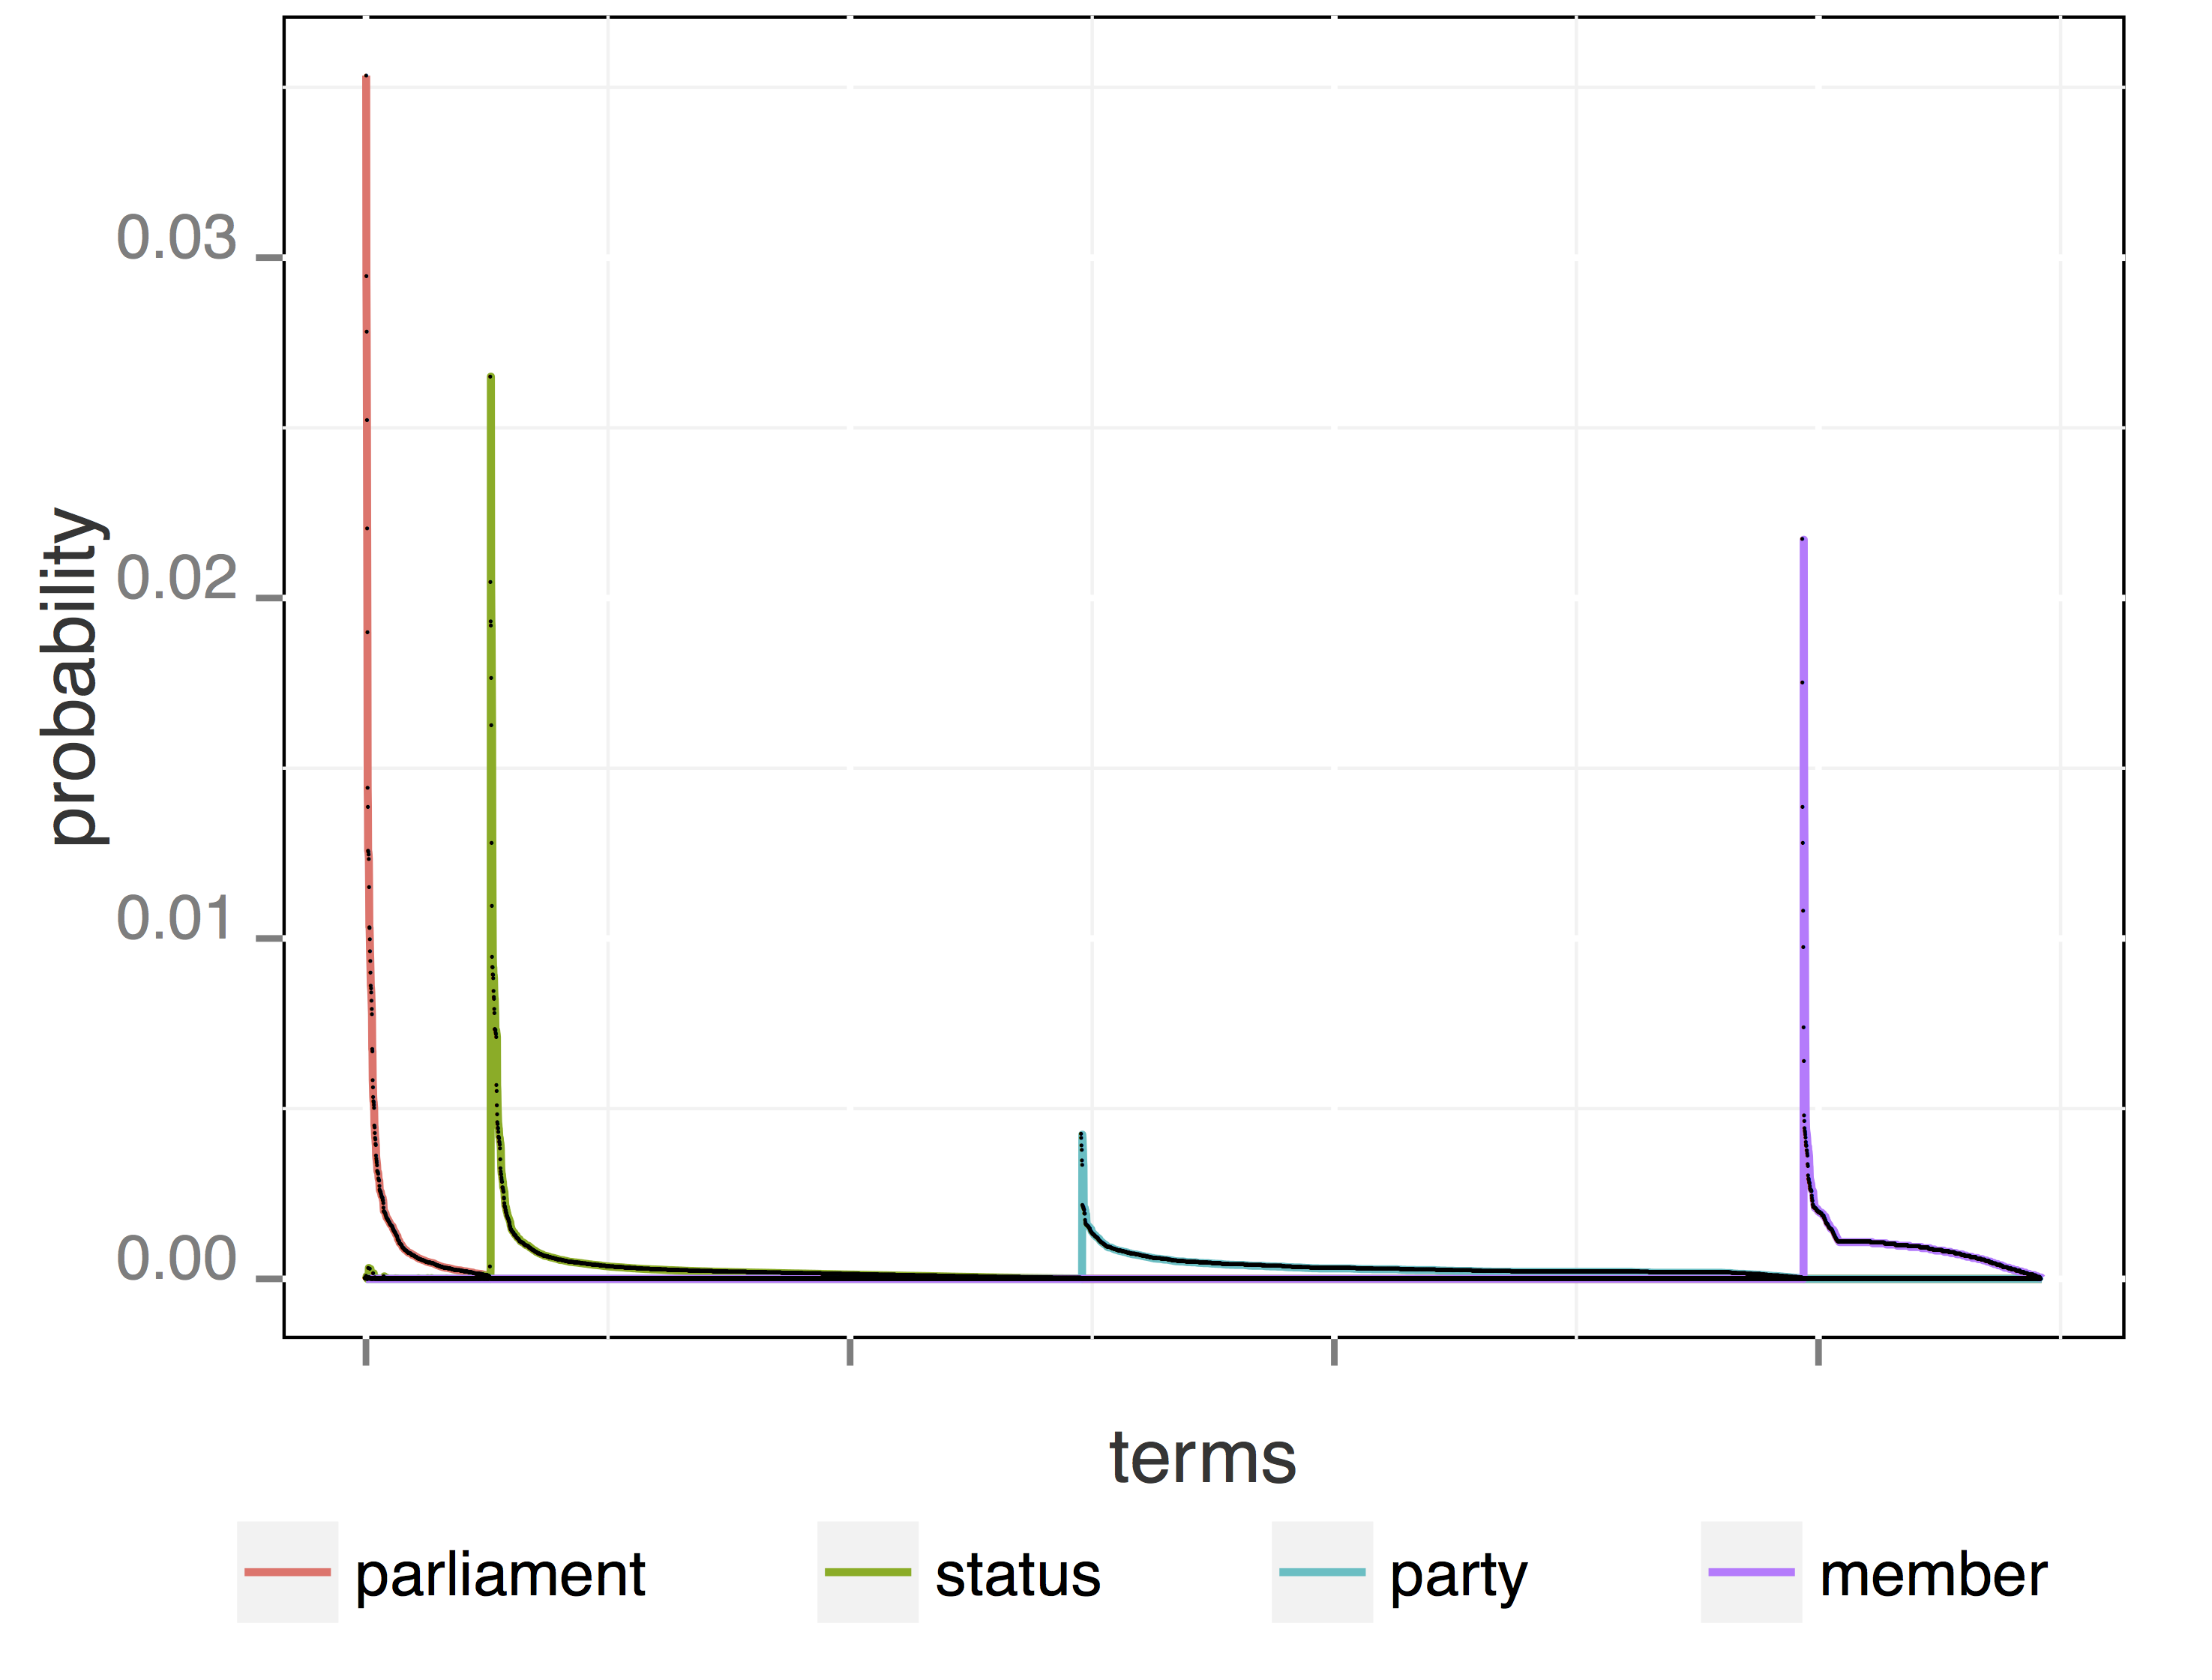
\includegraphics[width=\linewidth]{02-part-01/chapter-03/figs_and_tables/img_nlm02316.png}
\caption{\label{fig:VSO} \achswlm of S. van Haersma Buma (as the member of parliament - Leader of CDA), Christian Democratic Appeal (as the party), Opposition (as the status), and the Parliament}
        \end{subfigure}
        ~~~~~~~~
        \begin{subfigure}[b]{0.45\textwidth}
\centering
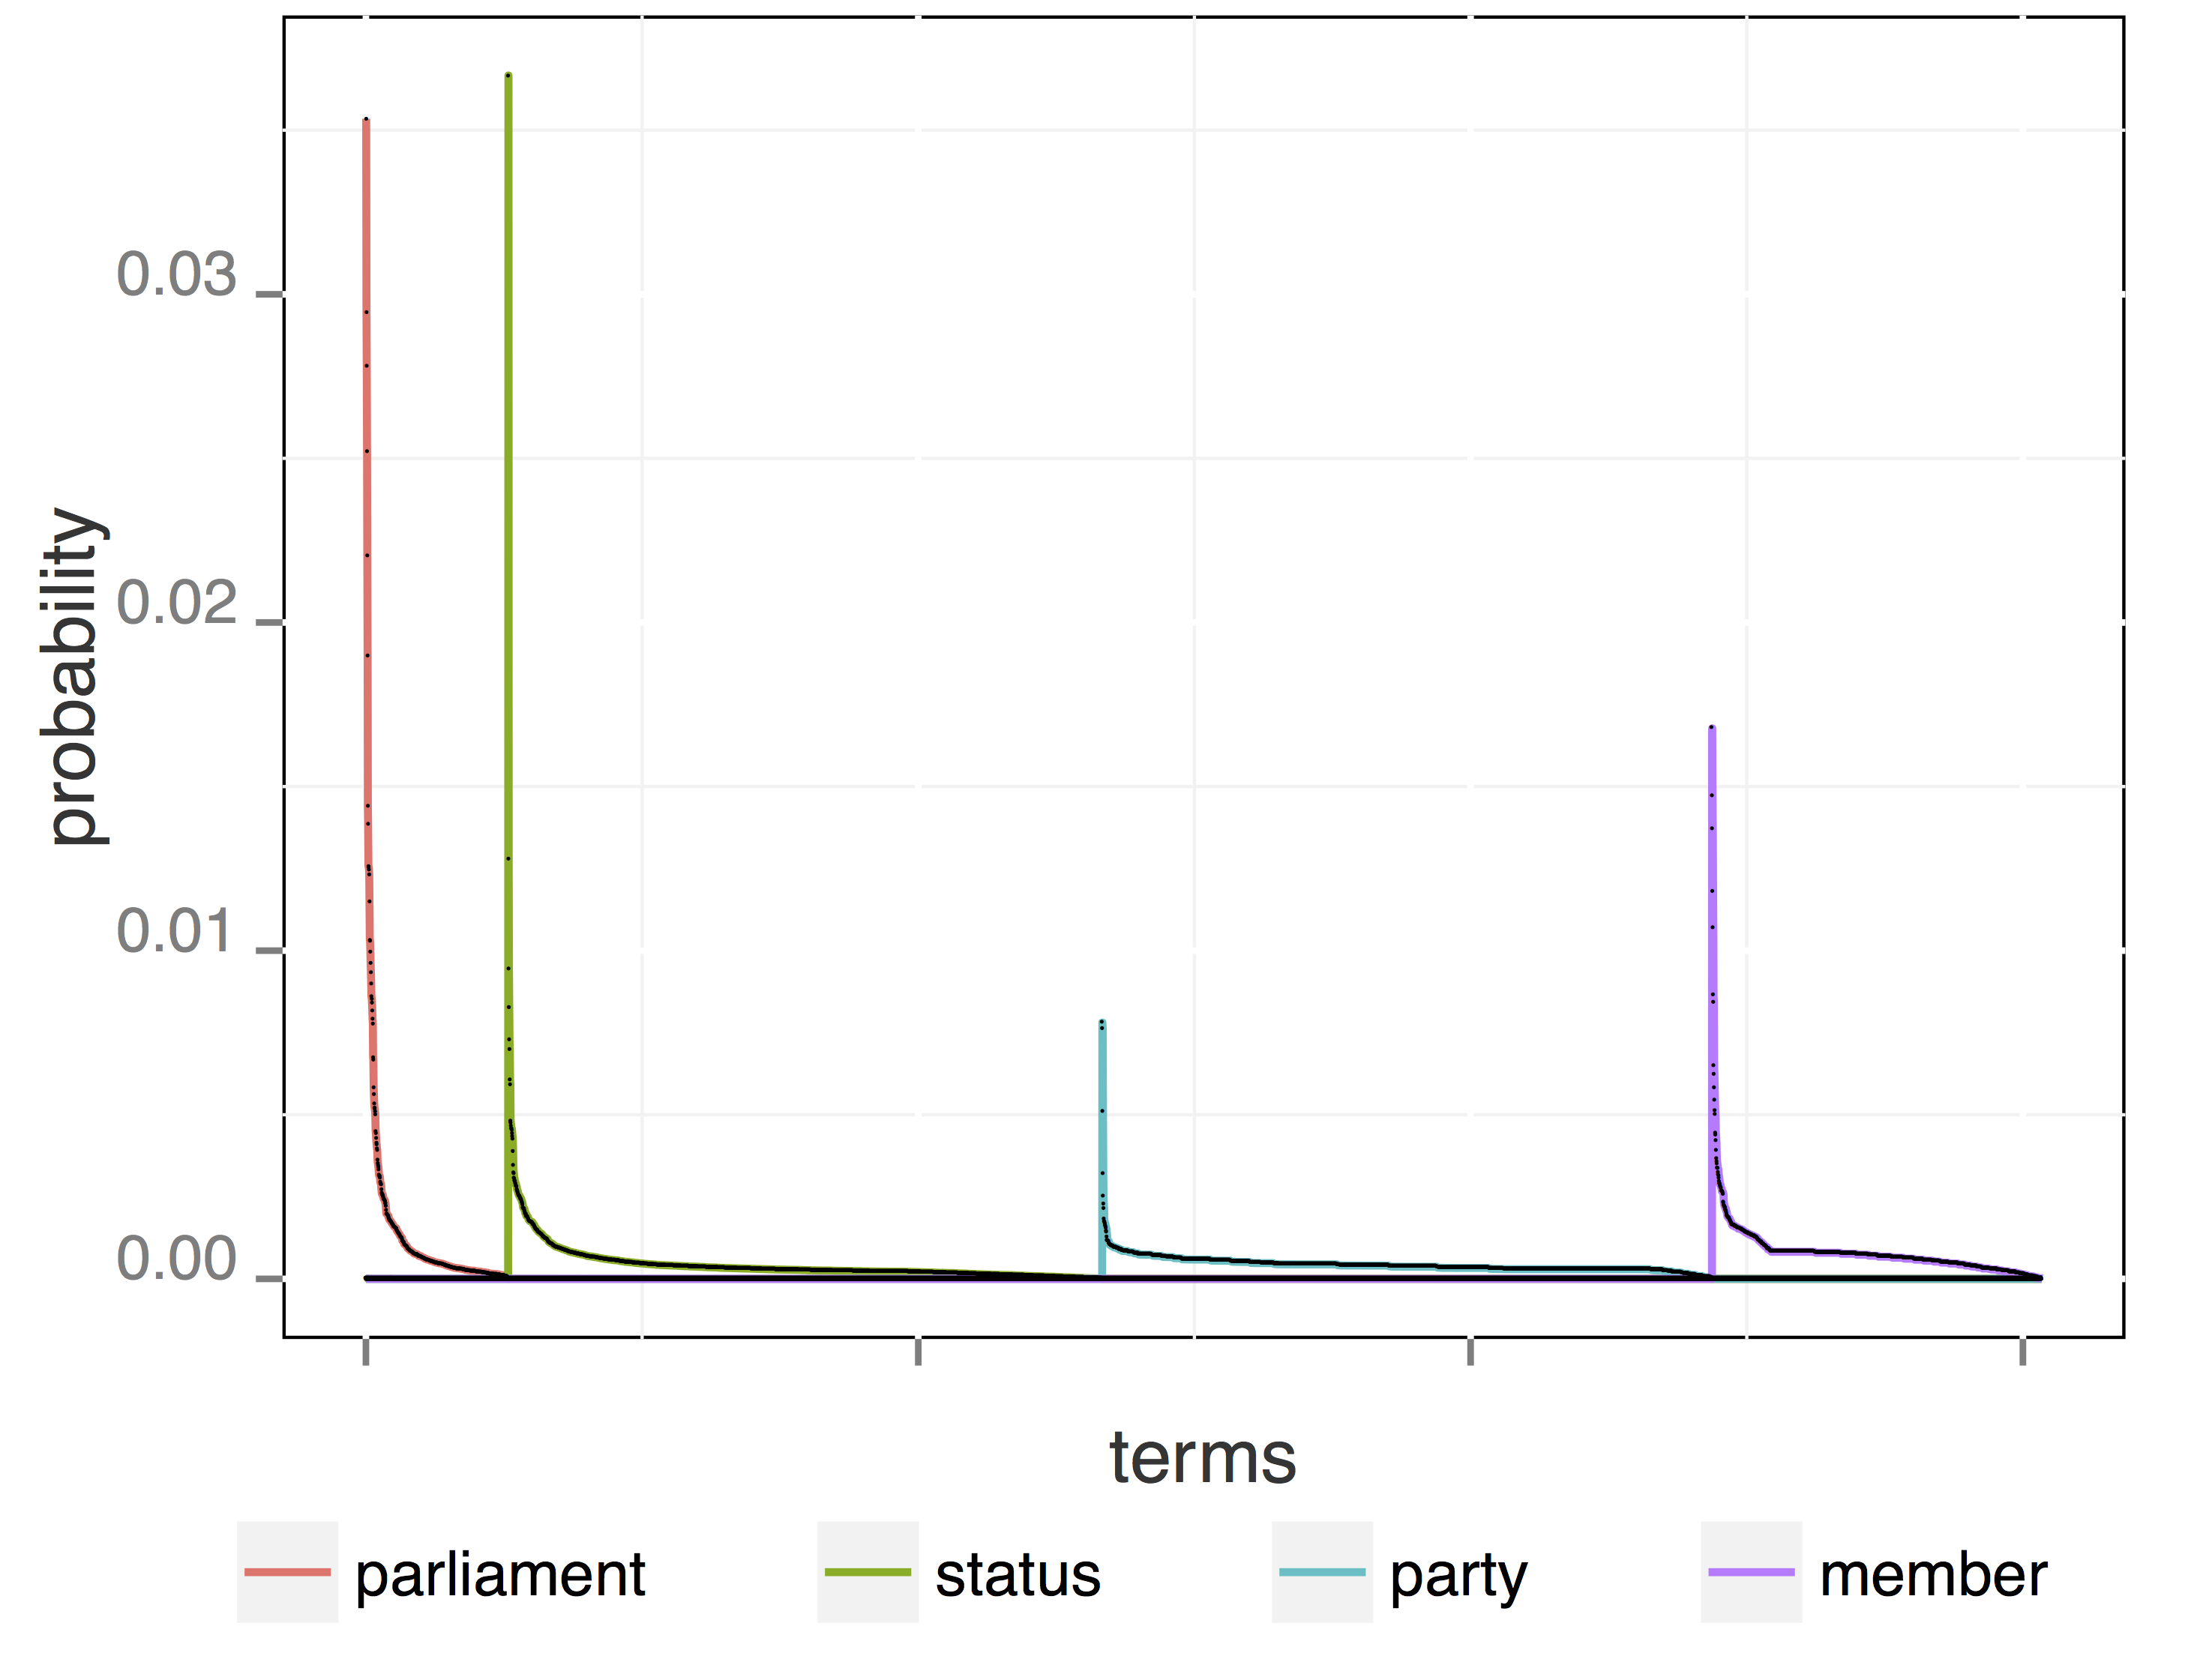
\includegraphics[width=\linewidth]{02-part-01/chapter-03/figs_and_tables/img_nlm02335.png}
\caption{\label{fig:VSC} \achswlm of D. Samson (as the member of parliament - Leader of PvdA), Labour Party (as the party), Government (as the status), and the Parliament}
        \end{subfigure}
        \caption{\label{fig:VS} \emph{Vertical Separability}: probability distribution over terms in different layers based on \hswlms in complete paths from the root to the terminal entities in the hierarchy}
\end{figure}

Two-dimensional separation property of \achswlm in the hierarchy is essentially due to the parsimonization effect in two directions. 
Intuitively, the horizontal separability is mainly the result of the specification stage. For example, when an entity is parsimonized given its direct parent, since the data in its parent is formed by pooling the data from the entity and its siblings, parsimonization makes the model of the entity separable from its siblings, which provide \emph{horizontal separation} in the resulting language models. On the other hand, vertical separability is mainly due to the generalization stage (and implicitly specification). For example, when an entity is parsimonized given its children, since they are specified already, parsimonization gets rid of the specific terms of the lower layer from the entity's model.


%---------------------------------------
\subsection{Separability for Transferability}
\label{subsec:Separability}
%---------------------------------------
As an extrinsic evaluation of the \hswlms, we investigate the effectiveness of the learned representations in a classification task in the parliamentary dataset with an evolving hierarchical structure. The task is to predict either the party that a member of the parliament belongs to, or the status of the member's party, having all the speeches given by that member in a period,  as well as all the speeches given by the members of all parties in a different period of parliament.

In the parliament, the composition of parties and statuses changes over different periods (Figure~\ref{fig:DutchParl}) and hence the speeches related to different entities can vary dramatically.  Due to this fact, cross-period classification is notoriously challenging \citep{Hirst:2014,yu:2008}.  We show that representing entities with \achswlm tackles the problem of having non-stable models when the composition of parliament evolves during the time, by capturing the essence of language models of parliamentary entities at aggregate levels. 

We use SVM as the base classifier and use the standard SVM as well as a SVM for training which we consider probabilities of terms in \achswlm as the weights of features in order to evaluate the effectiveness of \achswlm. Using the probabilities estimated by \achswlm as weights for features can be considered as a feature selection approach that filters out features that are not essential in accordance to the hierarchical position of entities and make the data representation more robust by taking out non-stable terms\footnote{We have also tried SVM along with a feature selection methods~\citep{Forman:2003,brank:2002} that uses the Information Gain (IG) to select features as a baselines and reported the results in~\citep{Dehghani:2016:ICTIR}.}.
We have employed conventional 5-fold cross validation for training and testing and to maintain comparability, we have used the same split for folding in all the experiments.

\begin{table}[!t]
\caption{Results on the task of party classification.}
\makebox[\linewidth][c]{
\centering
\begin{subtable}[b]{0.48\textwidth}
\captionof{table}{\label{tbl:SVM-party}Accuracy of the SVM classifier.}
\begin{adjustbox}{max width=\textwidth}
\begin{tabular}{ c l l l l l} \toprule
\multicolumn{2}{ c }{\multirow{2}{*}{\textbf{Period}}} & \multicolumn{4}{ c }{\textbf{Test}}
\\  \cmidrule{3-6}
\multicolumn{1}{ c}{} & & \textit{2006-10}& \textit{2010-12}& \textit{2012-14} & \textit{All}
\\ \midrule
\multirow{4}{*}{\rotatebox[origin=c]{90}{\textbf{Train}}} & \textit{2006-10} & \tc 47.56 & 29.22 & 26.84 & -
\\  
& \textit{2010-12} & 29.87 & \tc 40.90 & 35.57 & -
\\   
& \textit{2012-14} & 31.09 & 30.51 & \tc 44.96 & -
\\   
& \textit{All} & - & - & - & \tc 39.18
\\\bottomrule
\end{tabular}
\end{adjustbox}
\shrink
\end{subtable}
%
~~
%
\begin{subtable}[b]{0.48\textwidth}
\captionof{table}{\label{tbl:swlm-party}Accuracy of the $SVM_{\achswlm}$ classifier.}
\begin{adjustbox}{max width=\textwidth}
\begin{tabular}{ c l l l l l } \toprule
\multicolumn{2}{ c }{\multirow{2}{*}{\textbf{Period}}} & \multicolumn{4}{ c }{\textbf{Test}}
\\  \cmidrule{3-6}
\multicolumn{1}{ c}{} & &2006-10&2010-12&2012-14 & All
\\ \midrule
\multirow{4}{*}{\rotatebox[origin=c]{90}{\textbf{Train}}} & 2006-10 & \tc 44.51 & 46.10 & 43.62 & -
\\  
& 2010-12 & 40.85 & \tc 40.25 & 39.59 &-
\\   
& 2012-14 & 40.24 & 38.96 & \tc 42.28 & -
\\   
& All & - & - & - & \tc 49.94
\\\bottomrule
\end{tabular}
\end{adjustbox}
\end{subtable}
}
\end{table}

\newcolumntype{Y}{>{\centering\arraybackslash}X}
\begin{table}[!t]
\fontsize{7}{8}\selectfont
%\newcolumntype{Y}{>{\centering\arraybackslash}X}
\caption{Results on the task of status classification.\vspace{-10pt}}
\makebox[\linewidth][c]{
\centering
\begin{subtable}[b]{0.5\textwidth}
\captionof{table}{\label{tbl:SVM-status}Accuracy of the $SVM$ classifier}
\begin{tabular}{ c l l l l l } 
\toprule
\multicolumn{2}{ c }{\multirow{2}{*}{\textbf{Period}}} & \multicolumn{4}{ c }{\textbf{Test}}
\\ \cmidrule{3-6}
\multicolumn{1}{ c}{} & &2006-10&2010-12&2012-14 & All
\\ \midrule
\multirow{4}{*}{\rotatebox[origin=c]{90}{\textbf{Train}}} & 2006-10 & \tc 84.14 & 68.83 & 87.24 & -
\\ 
& 2010-12 & 68.29 & \tc 78.57 & 87.91 & -
\\
& 2012-14 & 68.90 & 75.97 & \tc 88.59 & -
\\ 
& All & - & - & - & \tc 79.87
\\\bottomrule
\end{tabular}
\shrink
\end{subtable}
%
~~~
%
\begin{subtable}[b]{0.5\textwidth}
\captionof{table}{\label{tbl:swlm-status}Accuracy of the $SVM_{\achswlm}$ classifier}
\begin{tabular}{ c l l l l l } \toprule
\multicolumn{2}{ c }{\multirow{2}{*}{\textbf{Period}}} & \multicolumn{4}{ c }{\textbf{Test}}
\\  \cmidrule{3-6}
\multicolumn{1}{ c}{} & &2006-10&2010-12&2012-14 & All
\\ \midrule
\multirow{4}{*}{\rotatebox[origin=c]{90}{\textbf{Train}}} & 2006-10 & \tc 82.32 & 80.51 & 89.29 &-
\\  
& 2010-12 & 79.87 & \tc 74.66 & 88.58 &-
\\   
& 2012-14 & 78.65& 77.27 & \tc 93.28 & -
\\   
& All & - & - & - & \tc 86.98
\\\bottomrule
\end{tabular}
\end{subtable}
}
\end{table}


Tables~\ref{tbl:swlm-status} and~\ref{tbl:swlm-party} show the performance of employing \acswlm on status and party classification respectively. 
Tables~\ref{tbl:SVM-status} and~\ref{tbl:SVM-party} indicate the results of SVM classifier on status and party classification respectively. Comparing the results in Tables~\ref{tbl:swlm-status} and~\ref{tbl:SVM-status}, we see that the accuracy of SVM in within period experiments is sometimes slightly better, but in cross period experiments, the classifier which uses \acswlm of statuses achieves better results.  This is also observed in the results in Table~\ref{tbl:swlm-party} compare to the results in Table~\ref{tbl:SVM-party}. 
%

For party classification, employing \acswlm results in a more significant improvement over the baseline.  \citet{Hirst:2014} discuss that since the status of members in parliament, compared to their party, has more effect on the content of their speeches, classifiers tend to pick features related to the status, not the party ideologies. So, SVM performs very well in terms of accuracy in the within-period experiments, but this performance is indebted to the separability of parties due to their status. Hence, changing the status in cross period experiments, using the trained model on other periods fails to predict the party, so the accuracies drop down. This is exactly the point which the strength of our proposed method kicks in. 
Since for each party, the \acswlm is less affected by the status of the party in that period, the model remains valid even when the status is changed.  In other words, eliminating the effect of the status layer in the party model in the specification stage ensures that the party model captures the essential terms related to the party ideology, not its status. Thereby, it is a stable model which is transferable through time.
%
We conducted the one-tailed t-test on the results. In both party and status classification, in all cases which \acswlm\ performs better than the SVM, the improvement is statistically significant ({p-value} $<$ 0.005).

To get a better intuition of the procedure of estimating \acswlm, consider the hierarchical relations of Dutch parliaments in the period of \emph{2006-2010} which is depicted in Figure~\ref{fig:DutchParl}. 
%
Assume that the goal is modeling language usage of ``Christian-Union (CU)'' as an entity in the party layer. In the speeches from the members of this party, words like ``\emph{Chairman}" or ``\emph{Agree}'' might occur repeatedly. However, they are not a good point of reference for the party's ideological language usage. In the procedure of estimating \acswlm\ of the "Christian-Union", these words are removed from the initial estimated standard language model in the specification stages, since ``\emph{Chairman}" is a general term in the parliamentary domain and is only able to explain the root entity and ``\emph{Agree}' is somehow an indicator of language usage of all the ``Government'' parties.
%
On the other side, consider the goal is to model language usage of ``Government'' as an entity in the status layer. Speeches from ``Christian-Union'' members, which are also counted as ``Government'' members, may contain words like ``\emph{Bible}'' or ``\emph{Charity}''.  It is trivial that involving these party-specific words in the constructed model for the ``Government'' in an individual period demolishes the comprehensiveness. In the procedure of estimating \acswlm\ for the ``Government'', in the generalization stages, these words are discarded from the model. This way, ``Government'' model does not lose its validity on other periods where the ``Christian-Union" is not in a Government party.

As another indicator of the effectiveness of \acswlm, it outperforms the SVM bringing all the data together from three different periods in both party and status classification. This is because it gets the chance of having richer train data which leads to more precise models. While in SVM, changes in the parliamentary composition make speeches diverse, and this makes it not to be able to learn a concrete model. 
\subsection{Invariance of the Representations}
\begin{figure}[!t]
\centering
\resizebox{0.9\linewidth}{!}{%
\begin{tikzpicture}
\pgfkeys{
     /pgf/number format/precision=2, 
    /pgf/number format/fixed zerofill=true,
    /pgf/number format/fixed
}
\begin{axis}[
    width= 12cm, %\textwidth,
    height=5cm, %5cm,
    ybar,%=0pt,
    ymajorgrids,
    minor tick num=1,
    bar width= 6.5pt,
    enlarge y limits=0.25,
    symbolic x coords={
    VVD,
    PvdA,
    CDA,
    PVV,
    SP,
    D66,
    CU,
    GL,
    Opposition,
    Government
},
    x tick label style={rotate=45,anchor=east},
    xtick=data,
    % ymin=0.0, 
    % ymax=0.5,
    ytick = {0.00,0.10,0.20,0.30,0.40,0.50},
    ylabel={},
    %legend style={at={(0.9,0.95),font=\fontsize{5}{6}},
    anchor=north,
    ylabel={JS-Divergence},
%    legend style={at={(0.65,-0.2),font=\fontsize{5}{6}},
    legend style={at={(0.965,0.95),font=\fontsize{5}{6}\selectfont},
    legend columns=1
    },
    nodes near coords,
    every node near coord/.append style={font=\fontsize{3}{4}\selectfont, rotate=90, anchor=west},
    %nodes near coords align={vertical},
    tick label style={font=\fontsize{5}{6}\selectfont}
    ]
\definecolor{b}{HTML}{3399FF}
\definecolor{g}{HTML}{5C7C19}
\addplot[fill=b, draw=b] coordinates
{
(VVD,0.3422)
(PvdA,0.3917)
(CDA,0.3889)
(PVV,0.2422)
(SP,0.3050)
(D66,0.2979)
(CU,0.4336)
(GL,0.4471)
(Opposition,0.1562)
(Government,0.2471)
};

\addplot[fill=g, draw=g, pattern color = g, pattern = north west lines] coordinates
{
(VVD,0.1639)
(PvdA,0.1631)
(CDA,0.1666)
(PVV,0.1641)
(SP,0.1918)
(D66,0.1890)
(CU,0.1757)
(GL,0.2759)
(Opposition,0.0512)
(Government,0.0759)
};

\legend{SLM,\acswlm}

\end{axis}
\end{tikzpicture}
}
\vspace{-12pt}
\caption{
Average of JS-Divergence of standard language models and {\acswlm}s for parliamentary entities in three different periods.\label{fig:cross_period_party_rep_divergence}}
 \vspace{-10pt}
 \end{figure}

As an intrinsic evaluation of the models, we evaluate the invariance of representations learned by our model over different periods---how similar are models of a particular in the hierarchy when trained on data from different periods. 
%
Since \achswlm is supposed to capture the essence of entities, not only \achswlm of an entity learned using an individual period should be valid for representing the entity on other periods, but also models of the same entity learned on data from different periods should be invariant. 

To assess this, we use the diversity of entities' models in different periods to measure their (in)variance over time.
%
First, all \achswlm from different periods of each party and each status is smoothed using Jelinek-Mercer smoothing \citep{Zhai:2001} considering all parliamentary speeches in the corresponding period as the background collection and with the same value of the smoothing parameter. Then, we use the Jensen-Shannon divergence as the diversity metric to measure dissimilarities between each two {\achswlm}s learned from different periods and then calculate the average of values for each entity. As the baseline, the same calculation is done for the standard language models of entities, i.e., language models estimated using maximum likelihood estimation. 
Figure~\ref{fig:cross_period_party_rep_divergence} shows the diversity of models in different periods.
%
As can be seen, in all entities in both party and status layers, diversity of \achswlm of different periods is lower than diversity of standard language models, which shows the extracted {\achswlm}s are more invariant over different periods. 


In order to better understand the results in the previous section, we zoomed in on the period of 2010-12 and 2012-2014 and looked into the confusion matrices of cross-period experiments and observed that most of the errors made by SVM are misclassifying members of CDA to PvdA and vice versa. These are the two parties that their statuses have been changed in these periods.  

\pgfplotstableread{
0    0.4801  0.8616  0.7492  
1    0.5667  0.5941  0.2422
2    0.3422  0.3222  0.6822
}\dataset

\definecolor{b}{HTML}{4981CE}
\definecolor{g}{HTML}{859C27}
\definecolor{r}{HTML}{B22222}
\definecolor{o}{HTML}{FF6600}

\begin{figure}[t]
\centering
\begin{tikzpicture}
\pgfkeys{
    /pgf/number format/precision=2, 
    /pgf/number format/fixed zerofill=true,
    /pgf/number format/fixed
}
\begin{axis}[
    width= 8.4cm, %\textwidth,
    height=5.7cm, %5cm,
    enlarge y limits=0.0,
    enlarge x limits=0.2,
    ymajorgrids,
    minor tick num=1,
    ybar,%=0pt,,
    bar width= 12pt,
    xtick=data,
    xticklabel style = {font=\fontsize{7}{8}\selectfont, align=center, text width=1.8cm},
    xticklabels = {Different Parties Same Period, Same Party Different Periods, Different Parties  Different Periods},
    ymin=0.0, 
    ymax=1.0,
    ytick = {0.00,0.10,0.20,0.30,0.40,0.50,0.60,0.70,0.80,0.90, 1.0},
    label style = {font=\fontsize{7}{8}\selectfont, yshift=0.5ex},
    anchor=north,
    ylabel={JS-Divergence},
    legend style={at={(0.965,0.95),font=\fontsize{5}{6}\selectfont},
    legend columns=-1
    },
    nodes near coords,
    every node near coord/.append style={font=\fontsize{5}{6}\selectfont, rotate=90, anchor=west},
    tick label style={font=\tiny},
    ]

\addplot[fill=b, draw=b, pattern color = b, pattern = north east lines] table[x index=0,y index=1] \dataset; 

\addplot[fill=r, draw=r, pattern color = r, pattern = dots] table[x index=0,y index=3] \dataset; 

\legend{TF,\achswlm}

\end{axis}
\end{tikzpicture}
\caption{
Average diversity of the representation of features of CDA and PvdA in different situations.}
\label{fig:cross_period_rep_divergence}
 \end{figure}

We investigate representations of these two parties to understand how separation in the feature representation affects the performance of cross period classification. To do so, for each of these two classes, in each period, we extract three probability distributions on terms indicating their importance based on different weighting approaches: 1) Term Frequency (used as feature weights in SVM) and 2) probability of terms in \achswlm (used as feature weights in $SVM_{\achswlm}$). 
Then, as a metric to measure separability of features, we use the Jensen-Shannon divergence to calculate diversity of probability distributions in three cases: 1) Different Parties in the Same Period, 2) Same Party in Different Periods 3) Different Parties in Different Periods. 
To avoid the effect of the number of features on the value of divergence, we take the top 500 high scored terms of each of the weighting methods as the fixed length representatives of them. Figure~\ref{fig:cross_period_rep_divergence} shows the average diversity of distributions in each of the three cases for each of the three weighting methods.

As expected, the diversity of features for different parties in a same period is high for both methods. However, when we calculate the diversity of features for a same party in different periods, feature representations are different in  $TF$, which causes false negative errors in the classification of these two parties. An interesting observation is in the case of having different parties in different periods, while we have two different parties their feature representations are similar in $TF$, which leads to false positive errors in the classification. 

Considering these observations together reveals that SVM learns representations on the basis of features that are indicators of issues related to the status of parties, since they are the most discriminating terms considering one period and in within period experiments, the performance of SVM is indebted to the separability of parties based on their statuses. Hence, after changing the status in the cross period experiments, the trained model of the previous period generated by SVM fails to predict the accurate party.  In the same way, the status classifier is affected by different parties forming a government in different periods, leading to lower accuracies.   

This is exactly the point which the strengths of \achswlm kicks in. In fact, two-dimensional separability in the feature representation, enables $SVM_{\achswlm}$ to tackle the problem of having non-stable features in the model when the status of a party changes over time. In other words, eliminating the effect of the status layer in the party model, which is the result of the horizontal separation, ensures that the party model captures the terms related to the party ideology, not its status. Thereby, not only $SVM_{\achswlm}$ learns an effective model with acceptable accuracy in within period experiments, but also its learned models remain valid when the statuses of parties change. 

\section{Related Work}
This section discusses briefly the separation property in the related domains and review principles in information retrieval and text classification, which are associated with the concept of separability.  
In addition, some research on classification and topic modeling of hierarchical texts are discussed. 

Separability is a property which makes the data representation sufficient to distinguish instances and consequently enables autonomous systems to easily interpreter the data~\citep{Lewis:1992}. For instance in the classification task, classifiers learn more accurate data boundaries when they are provided with separable representations of data from different classes~\citep{Lewis:1995}. The importance of separability in classifiers has led to the fact that making data separable becomes part of classification. As the most familiar instances, SVM by adding extra dimensions implicitly transform the data into a new space where they are linearly separable~\citep{Burges:1998}.

Separation is also a pivoting concept in the information retrieval. Separating relevant from non-relevant documents is a fundamental issue in this domain~\citep{Robertson:1977,saracevic:1975,Lavrenko:2001}. In IR, separation plays more important role when instead of giving a rank list, a decision should be made about relevancy of documents, for example in the information filtering task~\citep{Lewis:1992}. As another instance, in the task of relevance feedback, there are some efforts on estimating a distinctive model for relevant documents so that it reflects not only  their similarity, but also their difference from whole collection, i.e., what makes them stand out or separated~\citep{Sparck:2003,Hiemstra:2004,Zhai:SMM:2001}. 

In this chapter, we address the separation property in the textual data that are organizable in a hierarchical structure. In a hierarchy, due to the existence of dependencies between entities, estimating separated models is a complex task. There is a range of work on the problem of hierarchical text classification~\citep{Sebastiani:2002, Sun:2001}, which tried to model hierarchical text-based entities. \citet{McCallum:1998} proposed a method for modeling an entity in the hierarchy which tackles the problem of data sparseness in lower layer entities. They used a shrinkage estimator to smooth the model of each leaf entity with the model of its ancestors to make the models more reliable. 
There is also similar research on XML data processing, as hierarchically structured data, which try to incorporate evidence from other layers as the context through mixing each element language models by its parent's models~\citep{sigurbjornsson:2004,ogilvie:2004}.
%Their method in fact balances a trade-off between specificity and reliability. Although estimates in the leaf entities are more specific, due to data sparseness in these entities, the estimations are less reliable. Further up the hierarchy, there are more data instances so estimates are more reliable but unspecific.
%
%Later, \citet{Oh:2011}, similar to \citeauthor{McCallum:1998} tried to involve global information beside the local entity data to estimate the model of the entity. However, concerning large scale hierarchies, their method dynamically controls the level of information that is needed to be gathered from ancestors.

Recently, \citet{Song:2014} tackled the problem of representing hierarchical entities with a lack of training data for the task of hierarchical classification.  In their work, given a collection of instances and a set of hierarchical labels, they tried to embed all entities in a semantic space, then they construct a semantic representation for them to be able to compute meaningful semantic similarity between them.
%
%By focusing on scalability, \citet{Gopal:2013}, presented a framework which uses regularization technique for classifying entities with hierarchical and graphical dependencies to handle training data sparseness. They considered that the nearby entities in the hierarchy share similar model parameters and recursively push the parameters of the model of a node to be similar to its parents. This way, they encourage models of siblings to be similar to each other. 
%Again, their goal is to leverage information across the hierarchy that could be beneficial in case of training data sparseness. 

\citet{Zhou:2011} proposed a method that directly tackles the difficulty of modeling similar entities at lower levels of the hierarchy. They used regularization so that the model of lower level entities have the same general properties as their ancestors, in addition to some more specific properties. 
%
Although these methods tried to model hierarchical texts, but their concerns were not making the models separable. Instead, they mostly addressed the problem of \emph{training data sparseness} \cite{Ha-Thuc:2011,Song:2014,McCallum:1998} or presenting techniques for \emph{handling large scale data} \cite{Gopal:2013,Oh:2011,Xue:2008,Ha-Thuc:2011}.

In terms of modeling hierarchical entities, \citet{Kim:2013} used Hierarchical Dirichlet Process \citep[HDP,][]{Teh:2006} to construct models for entities in the hierarchies using their own models as well as the models of their ancestors.  Also, \citet{Zavitsanos:2011} used HDP to construct the model of entities in a hierarchy employing the models of its descendants. This research tries to bring out precise topic models using structure of the hierarchy, but they do not aim to estimate separable models.  

As we discussed in Section~\ref{subsec:Separability}, our proposed approach can be employed as a feature selection method for text classification. Prior research on feature selection for textual information~\citep{SIGIR-Workshop-2010,Forman:2003} tried to improve classification accuracy or computational efficiency, while our method aims to provide a separable representation of data that helps train a transferable model. 
Apart from considering the hierarchical structure, our goals also differ from prior research on transferability of models. For instance, research on constructing dynamic models for data streams~\citep{Yao:2009,Blei:2006} first discovered the topics from data and then tried to efficiently update the models as data changes over the time, while our method aims to identify tiny precise models that are more robust and remain valid over time.  Research on domain adaptation~\citep{Xue:2008:plsa,Chen:2011} also tried to tackle the problem of missing features when very different vocabulary are used in test and training data.  This differs from our approach considering the hierarchical relations, as we aim to estimate separable models that are robust against changes in the structure of entities relations, rather than changes in the corpus vocabulary.


\section{Conclusion}
Building conceptually accurate models of data with a structure consisting of multiple layers, or a hierarchy, prompts us to analyze them at different abstraction levels.  However, this requires the ability to estimate separable models for hierarchical entities which capture their essential features taking into account their relative position in the hierarchy. 

In this chapter, we demonstrated that based on the ranking and classification principles, the \emph{separation property} in the data representation is a desirable foundational property which leads to separability of scores and consequently improves the accuracy of classifiers' decisions.  We stated this as the ``\ssp'' for optimizing expected effectiveness of classifiers.

We showed that in order to have horizontally and vertically separable models, they should capture all, and only, the essential terms of the entities taking their position in the hierarchy into account. Based on this, we introduced \hswlms for estimating separable models for hierarchical entities. We studied \achswlm and demonstrated that it offers separable distributions over terms for different entities both in case of being in the same layer or in different layers.  We evaluated the performance of classification over time using separable representations of data and showed that separability makes the model more robust and transferable over time by filtering out non-essential non-stable terms.

%connection to part 2
In this part of the thesis, we studied how taking the structure of the data into account can help learning more robust representations against noisy and variant factors of the data. In Part~\ref{part3}, we investigate how we can change the learning process to make it more robust against the noise in the weakly annotated labels.